\documentclass[12pt,a4paper]{article}
\usepackage[T1]{fontenc}
\usepackage[utf8]{inputenc}
\usepackage{geometry}
\usepackage{float}
\usepackage{graphicx}
\usepackage{wrapfig}
\usepackage{setspace}
\usepackage{xcolor}
\usepackage{gensymb}
\usepackage{amsmath,mathtools,breqn, amsfonts}

\geometry{a4paper,left=2cm,right=2cm}

\clearpage

\begin{document}
	\begin{titlepage}
		\centering
		\vspace*{\fill}
		{\scshape\LARGE Università degli Studi di Verona \par}
		\vspace{1.5cm}
		
\includegraphics[scale=0.5]{./images/univr_logo.png}
		\vspace{1.5cm}\\
		\line(1,0){145} \\
		{\huge\bfseries Sistemi\par}
		\line(1,0){145} \\
		\vspace{0.5cm}
		{\scshape\Large Eserciziario\par}
		\vspace{2cm}
		{\Large Magdalena M. Solitro\par}
		\vspace{1cm}
		
		\vspace{5cm}
		\vspace*{\fill}
		% Bottom of the page
		{}
		{\large \today\par}
	\end{titlepage}
	\thispagestyle{empty}
	
	\section*{Sistemi LTI a tempo continuo}
	\paragraph*{Esercizio 1.1}
	Si consideri il sistema dinamico rappresentato dalla seguente equazione differenziale:
	\[
		\begin{cases}
   		\ddot{v}(t) + 5\dot{v}(t) + 4v(t) = \dot{u}(t) - bu(t) \\
   		\dot{v}(0) = 1 \\
   		v(0) = 0 \\
   		u(t) = e^{-2t} \delta_{-1}(t) \\
   		\end{cases}
   	\]
   	\begin{enumerate}
   		\item Deteterminare la stabilit\'a asintotica del sistema al variare di \textit{b}
   		\item Determinare l'evoluzione libera per \textit{b} = 1
   		\item Determinare la risposta impulsiva nel dominio delle frequenze (Laplace)
   		\item Determinare la risposta totale nel dominio delle frequenze (Laplace)
   	\end{enumerate}
   	-----------------------------------------------------------------------------------------------------------------------\\
   	\begin{enumerate}
   	\item Un sistema dinamico \'e \textbf{asintoticamente stabile} se e solo se tutte le sue radici caratteristiche si trovano nel semipiano negativo del piano complesso:
   	\[
   		\mathbb{R}e(s_1), \mathbb{R}e(s_2), ... , \mathbb{R}e(s_n) < 0
   	\]
   	Calcoliamo quindi le radici caratteristiche del sistema:
   	\[
   		s^2 + 5s + 4 = 0
   		\Longleftrightarrow
   		s_1 = -4, s_2 = -1
   	\]
   	Notiamo che sono radici reali negative, quindi il sistema\textbf{ è asintoticamente stabile} per qualunque valore di \textit{b}.\\
   	Dato che la stabilità asintotica implica la BIBO stabilità , possiamo dire che il sistema è anche \textbf{ BIBO stabile}, per qualunque valore di \textit{b}.
   	\item Per \textit{b} = 1, l'equazione del nostro sistema diventa:
   	\[
   	\ddot{v}(t) + 5\dot{v}(t) + 4v(t) = \dot{u}(t) - u(t)
   	\]
   	L'evoluzione libera del sistema è data dalla seguente espressione:
   	\[
   		v_l(t) = c_1e^{s_1t} + c_2e^{s_2t}
   	\]
   	\[
   		v_l(t) = c_1e^{-4t} + c_2e^{-t}
   	\]
   	Impongo le condizioni iniziali per ricavare i coefficienti $c_1$ e $c_2$:
	\[
   		\begin{cases}
   		v(0) = 0 = c_1 + c_2 \\
   		\dot{v}(0) = 1 = -4c_1 - c_2
   		\end{cases}
   	\]
   	Da cui ricaviamo che $c_1 = -\frac{1}{3}$ e $c_2 = \frac{1}{3}$
   	L'espressione finale dell'evoluzione libera risulta quindi essere:
   	\[
   		v_l(t) = -\frac{1}{3}e^{-4t} + \frac{1}{3}e^{-t}
   	\]
   	\item Scriviamo la funzione di trasferimento \textit{H(s)}:
   	\[
   		H(s) = \frac{s-1}{(s+4)(s+1)}
   	\]
   	Scompongo in fratti semplici:
   	\[
   	H(s) = \frac{A}{s+4} + \frac{B}{s+1}
   	\] \\
   	$ A = (s+4) \frac{s-1}{(s+4)(s+1)}\Bigl\vert_{s=-4} = \frac{5}{3} $ \\ \\
	$ B = (s+1) \frac{s-1}{(s+4)(s+1)}\Bigl\vert_{s=-1} = -\frac{2}{3} $ \\ \\
	Quindi l'espressione di \textit{H(s)} scomposta risulta essere:
	\[
		H(s) = \frac{5}{3}\frac{1}{s+4} -\frac{2}{3}\frac{1}{s+1}
	\]
   	Questa forma ci permette di calcolare agevolmente l'antitrasformata di Laplace, e arrivare quindi all'espressione finale della risposta impulsiva nel dominio del tempo:
   	\[
   		h(t) = \left(\frac{5}{3}e^{-4t}-\frac{2}{3}e^{-t}\right) \delta_{-1}(t)
   	\]
	\item Per calcolare la risposta totale del sistema nel dominio delle frequenze, devo eseguire la trasformata di Laplace sia dell'ingresso che dell'uscita:
	\[
		\mathcal{L}[\ddot{v}(t) + 5\dot{v}(t) + 4v(t)] = \mathcal{L}[\dot{u}(t) - u(t)]
	\]
	\vspace{5px}
	\[
		s^2V(s) - (0\cdot s^1+1\cdot s^0) + 5(s^1V(s)-0)+4s^0V(s) = sU(s) - U(s)
	\]
	\vspace{5px}
	\[
		V(s) (s^2 + 5s + 4) = U(s)(s-1) -1
	\]
	\vspace{5px}
	\[
		V(s) = U(s)\frac{s-1}{(s^2+5s+4)}-\frac{1}{(s^2+5s+4)}
	\]
	\vspace{5px}
	\\Dato che $u(t) = e^{-2t} \delta_{-1}(t)$, ricaviamo che $U(s) = \mathcal{L}[u(t)] = \frac{1}{s+2} $ , e quindi
	\[
		V(s) = \frac{s-1}{(s+4)(s+2)(s+1)}-\frac{1}{(s+4)(s+1)} = \frac{-3}{(s+4)(s+2)(s+1)}
	\]
	Applico il metodo dei fratti semplici:
	\[
		V(s) = \frac{A}{s+4}+\frac{B}{s+1}+\frac{C}{s+2}
	\]
	Ricavo i coefficienti A, B, C:\\ \\
	$A = (s+4)\frac{-3}{(s+4)(s+2)(s+1)}\Bigl\vert_{s=-4} = -\frac{1}{2}$\\ \\
	$B = (s+1)\frac{-3}{(s+4)(s+2)(s+1)}\Bigl\vert_{s=-1} = -1$\\ \\
	$C = (s+2)\frac{-3}{(s+4)(s+2)(s+1)}\Bigl\vert_{s=-2} = \frac{3}{2}$\\ \\
	Da cui ricaviamo l'espressione di V(s) scomposta:
	\[
		V(s) = -\frac{1}{2}\frac{1}{s+4}-\frac{1}{s+1}+\frac{3}{2}\frac{1}{s+2}
	\]
	Eseguendo l'antitrasformata di Laplace otteniamo l'espressione della risposta totale nel dominio del tempo:
	\[
		v(t) = \left(-\frac{1}{2}e^{-4t}-e^{-t}+\frac{3}{2}e^{-2t}\right)\delta_{-1}(t)
	\]
	\end{enumerate}
	\newpage
	\paragraph*{Esercizio 1.2 - parziale del 02/05/2019}
	Si consideri il seguente sistema dinamico rappresentato dall'equazione differenziale:
	\[
		\begin{cases}
			\ddot{v}(t) -5\ddot{v}(t) + 6v(t) = \ddot{u}(t) + \dot{u}(t) + (3+k)u(t)\\
			\dot{v}(0) = 2\\
			v(0) = 1\\
			u(t) = 2e^{4t}\delta_{-1}(t)
		\end{cases}
	\]
	\begin{enumerate}
		\item Discutere la stabilit\'a del sistema al variare del parametro k
		\item \textit{k = -5}: calcolare la risposta libera nel dominio del tempo
		\item Calcolare la risposta impulsiva nel \underline{dominio del tempo}
		\item Calcolare la risposta forzata utilizzando l'antitrasformata di Laplace
	\end{enumerate}
--------------------------------------------------------------------------------------------------------------------------\\
	\begin{enumerate}
		\item Dobbiamo verificare che tutte le radici caratteristiche dell'equazione differenziale siano \textit{minori di 0}:
		\[
			s^2-5s+6=0
			\Rightarrow
			s_1 = 3, s_2 = 2
		\]
		Il sistema, quindi \textbf{non è asintoticamente stabile}, e notiamo che questo non dipende dal parametro k.\\
		Dobbiamo quindi verificare esplicitamente l'eventuale stabilit\'a BIBO: il sistema risulta essere BIBO stabile se e solo se tutte le radici caratteristiche che causano l'instabilit\'a asintotica (in questo caso $s_1$ e $s_2$) si semplificano nella funzione di trasferimento.
		\[
			H(s) = \frac{s^2 + s + 3 + k}{s^2 - 5s +6}\\
		\]
		\[
			H(s) = \frac{s^2 + s + 3 + k}{(s-3)(s-2)}
		\]
		Le radici del polinomio al numeratore sono date da $\frac{-1\pm\sqrt{1-4(3+k)}}{2}$, quindi dovremmo trovare un $k$ univoco che possa essere soluzione del sistema:\\
		\[
			\begin{cases}
				\frac{-1+\sqrt{1-4(3+k)}}{2} = 3\\
				\frac{-1-\sqrt{1-4(3+k)}}{2} = 2
			\end{cases}
			\Rightarrow
			\begin{cases}
				k = -15\\
				\frac{-1-\color{red}\sqrt{-26}\color{black}}{2} = 2
			\end{cases}
		\]
		\\Nella seconda equazione abbiamo una radice negativa, quindi il sistema non ha soluzione!\\
		Non potendo fattorizzare il numeratore in modo da semplificare i poli, deduciamo che il sistema \textbf{non è BIBO stabile}.
		\item Ponendo k = -5, l'equazione differenziale che descrive il sistema diventa:
		\[
			\ddot{v}(t) -5\dot{v}(t) + 6v(t) = \ddot{u}(t) + \dot{u}(t) -2u(t)
		\]
		Sappiamo gi\'a dal punto precedente che le radici del sistema sono $s_1 = 3$ e $s_2 = 2$. Quindi:
		\[
			v_l(t) = c_1e^{3t} + c_2e^{2t}
		\]
		Non ci resta che trovare il valore dei coefficienti $c_1$ e $c_2$ imponendo le condizioni iniziali:
		\[
			\begin{cases}
				v(0) = 1\\
				\dot{v}(0) = 2
			\end{cases}
			\Rightarrow
			\begin{cases}
				c_1 + c_2 = 1\\
				2c_1 + 3c_2 = 2
			\end{cases}
			\Rightarrow
			\begin{cases}
				c_1 = 1\\
				c_2 = 0
			\end{cases}
		\]
		Giungiamo quindi all'espressione che descrive l'evoluzione libera:
		\[
			v_l = e^{2t}
		\]
		\item Scriviamo l'espressione generale della risposta impulsiva, tenendo conto del fatto che il sistema è \textit{proprio} e che dunque deve comparire il termine impulsivo:
		\[
			h(t) = d_0\delta(t)+(d_1e^{2t} + d_2e^{3t})\delta_{-1}(t)
		\]
		Nell'equazione originale sostituiamo $h(t)$ a $v(t)$, e $\delta(t)$ a $u(t)$:
		\begin{equation}
			\ddot{h}(t) - 5\dot{h}(t) + 6h(t) = \frac{d^2\delta(t)}{dt^2} + \frac{d\delta(t)}{dt} -2\delta(t)
		\end{equation}
		Scriviamo di seguito le derivate di primo e secondo ordine di $h(t)$:\\ \\
		\[
			\frac{d h(t)}{dt} = d_0\frac{d \delta(t)}{dt} + (2d_1e^{2t} + 3d_2e^{3t})\delta_{-1}(t) + (d_1e^{2t} + d_2e^{3t})\delta(t)
		\]
		\begin{align*}
			\frac{d^2h(t)}{dt^2} &= d_0\frac{d^2\delta(t)}{dt^2} + (4d_1e^{2t} + 9d_2e^{3t})\delta_{-1}(t) + 2(2d_1e^{2t}+ 3d_2e^{3t})\delta(t) \\& + (d_1e^{2t} + d_2e^{3t})\frac{d\delta(t)}{dt}
		\end{align*}
		Ora si sostituiscono queste espressioni nell'equazione (1) e si svolgono i calcoli (si possono omettere gli esponenziali, dato che siamo interessati solo ai valori dei coefficienti $d_0$, $d_1$ e $d_2$).
		Alla fine, l'equazione (1) dovrebbe risultare cos\'i:
		\[
			d_0\frac{d^2h(t)}{dt^2} + (-5d_0 + d_1e^{2t} + 9d_2e^{3t})\frac{d h(t)}{dt} + (6d_0 - d_1e^{2t} + d_2e^{3t}) = \frac{d^2h(t)}{dt^2} + \frac{d h(t)}{dt} - 2\delta(t)
		\]
		Ora dobbiamo fare in modo che i coefficienti dei termini a sinistra coincidano con quelli che erano presenti dell'equazione originale! Quindi impostiamo il seguente sistema:
		\[
			\begin{cases}
				d_0 = 1\\
				-5d_0 -d_1 + d_2 = 1\\
				6d_0 - d_1 + d_2 = -2
			\end{cases}
			\Rightarrow
			\begin{cases}
				d_0 = 1\\
				d_1 = 7\\
				d_2 = -1
			\end{cases}
		\]
		L'espressione definitiva della risposta impulsiva h(t) \'e:
		\[
			h(t) = \delta(t) + (7e^{2t} - e^{3t})\delta_{-1}(t)
		\]
		\item Nel dominio delle frequenze, invece, la risposta forzata si calcola come il prodotto della funzione trasferimento per la trasformata di Laplace dell'ingresso:
		\[
			V_f(s) = \mathcal{L}[h(t)*u(t)] = H(s)\cdot U(s)
		\]
		La proprietà di convoluzione della trasformata di Laplace dice infatti che se due funzioni $v_1(t)$ e $v_2(t)$ sono nulle per $t<0$ e sono dotate di trasformata di Laplace, rispettivamente $V_1(s)$ e $V_2(s)$, allora il prodotto di convoluzione $[v_1 * v_2](t)$ nel tempo diventa un prodotto semplice, $V_1(s)\cdot V_2(s)$ nelle frequenze.\\ Proseguiamo dunque nel calcolo della risposta forzata:
		\[
			V_f(s) = \frac{2s^2 + s - 2}{s^2 - 5s + 6}\cdot\frac{2}{s-4} = \frac{2s^2 + s - 2}{(s-3)(s-2)} \cdot \frac{2}{s-4}
		\]
		Scomposizione in fratti semplici:
		\[
			V_f(s) = \frac{A}{s-2}+\frac{B}{s-3}+\frac{C}{s-4}
		\]
		Calcoliamo quindi il valore dei vari coefficienti:\vspace{5px}\\
		$A = (s-2)\frac{2(2s^2+s-2)}{(s-2)(s-3)(s-4)}\Bigl\lvert_{s = 2} = 8$\vspace{5px}\\
		$B = (s-3)\frac{2(2s^2+s-2)}{(s-2)(s-3)(s-4)}\Bigl\lvert_{s = 3} = -38$\vspace{5px}\\
		$C = (s-4)\frac{2(2s^2+s-2)}{(s-2)(s-3)(s-4)}\Bigl\lvert_{s = 4} = 34$\vspace{5px}\\\\
		Quindi possiamo riscrivere l'espressione dell'evoluzione forzata come:
		\[
			V_f(s) = \frac{8}{s-2}+\frac{-38}{s-3}+\frac{34}{s-4}
		\]
		Ora possiamo facilmente ricavare il suo equivalente nel dominio del tempo applicando le antitrasformate elementari:
		\[
			v_f(t) = 8e^{2t}\delta_{-1}(t) -38e^{3t}\delta_{-1}(t) + 34e^{4t}\delta_{-1}(t)
		\]
	\end{enumerate}
	\newpage
	\paragraph*{Esercizio 1.3}
	Si consideri il seguente sistema dinamico rappresentato dall'equazione differenziale:
	\[
		\begin{cases}
			\ddot{v}(t) + 2\dot{v} + 5v(t) = \dot{u}(t) + u(t)\\
			\dot{v}(0) = 1\\
			v(0) = 1\\
			u(t) = 2\delta_{-1}(t)
		\end{cases}
	\]
	\begin{enumerate}
		\item Discutere la stabilit\'a asintotica
		\item Calcolare l'evoluzione libera del sistema
		\item Calcolare la risposta impulsiva nel \underline{dominio del tempo}
		\item Calcolare l'evoluzione forzata con il \underline{prodotto di convoluzione}
	\end{enumerate}
	---------------------------------------------------------------------------------------------------------------------------\\
	\begin{enumerate}
		\item L'equazione caratteristica del sistema \'e:
		\[
			s^2 + 2s + 5s = 0
		\]
		che ha due radici complesse: $s_1 = -1+2j$ e $s_2 = -1-2j$.\\
		Notiamo che $Re(s_1) < 0$ e $Re(s_2) < 0$, quindi il sistema \'e asintoticamente stabile.\\
		Di conseguenza, \'e anche BIBO stabile.
		\item Dato che le radici dell'equazione caratteristica sono complesse, l'evoluzione libera si presenta nella seguente forma:
		\[
			v_l = c_1e^{-t}cos(2t) + c_2e^{-t}sin(2t)
		\]
		L'occorrenza delle funzioni seno e coseno in presenza di radici caratteristiche complesse è una conseguenza dell'\textbf{identità di Eulero}:
		\[
			e^{i\pi} = cos(\pi) + i sin(\pi)
		\]
		$e^{i\pi}$ è il vettore che individua il numero nel piano complesso. Il suo modulo è costante, dunque localizza tutti i numeri complessi che stanno su una circonferenza di raggio pari a $|e^{i\pi}|$.\\
		Intuitivamente, nell'equazione dell'evoluzione libera la parte reale della radice è contenuta nell'esponente di $e$, mentre la componente complessa è nell'argomento del seno (o del coseno).\\
		Ora imponiamo le condizioni iniziali e ricaviamo il valore dei coefficienti.\\
		Attenzione al calcolo della derivata di $v_l$:\\
		$\dot{v}_l(t) = c_1e^{-t}(-cos(2t)-2sin(2t) + c_2e^{-t}(-sin(2t)+2cos(2t))$
		\[
			\begin{cases}
				v(0) = 1 = c_1e^0cos(0) + c_2e^0sin(0)\\
				\dot{v}(0) = 1 = c_1e^0(-cos(0)-sin(0)) + c_2e^0(cos(0)-sin(0))
			\end{cases}
			\Rightarrow
			\begin{cases}
				c_1 = 1\\
				c_2 = -\frac{1}{2}\\
			\end{cases}
		\]
		Quindi possiamo scrivere l'espressione finale dell'evoluzione libera:
		\[
			v_l(t) = e^{-t}cos(2t)-\frac{1}{2}e^{-t}sin(2t)
		\]
		\item Dato che il sistema è \textit{proprio} (ovvero: il massimo grado di derivazione dell'uscita \'e maggiore del massimo grado di derivazione dell'ingresso), l'espressione della risposta impulsiva sar\'a:
		\[
			h(t) = (d_1e^{-t}sin(2t) + d_2e^{-t}cos(2t))\delta_{-1}(t)
		\]
		Per ricavare i coefficienti $d_1$ e $d_2$, dobbiamo fare la derivata prima e seconda di $h(t)$ e sostituirle nell'equazione originale. Al posto degli ingressi, inoltre, dobbiamo sostituire l'impulso di Dirac.\\ \\
		\begin{align*}
			\frac{dh(t)}{dt} &= \left[-d_1e^{-t}cos(2t)-2d_1e^{-t}sin(2t)-d_2e^{-t}sin(2t) + 2d_2e^{-t}cos(2t)\right]\delta_{-1}(t)\\& + (d_1e^{-t}cos(2t) + d_2e^{-t}sin(2t))\delta_{-1}(t)
		\end{align*}
		\begin{align*}
			\frac{d^2h(t)}{dt^2} &= [d_1e^{-t}cos(2t)+2d_1e^{-t}sin(2t)+2d_1e^{-t}sin(2t)-4d_1e^{-t}cos(2t)+d_2e^{-t}sin(2t) \\&-2d_2e^{-t}cos(2t)-2d_2e^{-t}cos(2t)-4d_2e^{-t}sin(2t)]\delta_{-1}(t)+2[-d_1e^{-t}cos(2t)\\&-2d_1e^{-t}sin(2t)-d_2e^{-t}sin(2t)+2d_2e^{-t}cos(2t)]\delta(t) + (d_1e^{-t}cos(2t)+d_2e^{-t}sin(2t))\frac{d\delta(t)}{dt} 
		\end{align*}
		\\ \\
		Fortunatamente, molti dei termini presenti in queste espressioni si annullano tra loro!\\
		Dopo aver effettuato le opportune semplificazioni, rimaniamo con la seguente equazione:
		\[
			[-4d_1e^{-t}sin(2t)+4d_2e^{-t}cos(2t)]\delta(t) + [d_1e^{-t}cos(2t)+d_2e^{-t}sin(2t)]\frac{d\delta(t)}{dt} = \frac{d\delta(t)}{dt} + \delta(t)
		\]
		I coefficienti dei termini a sinistra devono coincidere con quelli dell'equazione originale, quindi:
		\[
			\begin{cases}
				d_1 = 1\\
				d_2 = \frac{1}{4}
			\end{cases}
		\]
		Ora inseriamo questi coefficienti nell'espressione iniziale della risposta impulsiva, ottenendo:
		\[
			h(t) = \left(e^{-t}cos(2t) + \frac{1}{4}e^{-t}sin(2t)\right)\delta_{-1}(t)
		\]
		\item La risposta forzata del sistema è definita come il prodotto di convoluzione tra la risposta impulsiva e l'ingresso:
		\[
			v_f(t) = \int_{0}^{+\infty}h(\tau)\cdot u(t-\tau)\; d\tau
		\]
		Ovvero:
		\begin{align*}
			v_f(t) &= \int_{0}^{+\infty}\left(e^{-\tau}cos(2\tau) + \frac{1}{4}e^{-\tau}sin(2\tau)\right)\delta_{-1}(\tau)\cdot2\delta_{-1}(t-\tau)\; d\tau\\& = 
			2\int_{0}^{+\infty} e^{-\tau}\left(cos(2\tau)+\frac{1}{4}sin(2\tau)\right)\;d\tau\\& = 
			2\left[\left(cos(2\tau) + \frac{1}{4}sin(2\tau)\right)(-e^{-\tau}) + \int_{0}^{+\infty}e^{-\tau}\left(-2sin(2\tau) + \frac{1}{2}cos(2\tau)\right)\;d\tau\right]\\& = 
			2\left[\int_{0}^{+\infty}e^{-\tau}cos(2\tau)\;d\tau + \frac{1}{4}\int_{0}^{+\infty}e^{-\tau}sin(2\tau)\; d\tau\right] \\&= 2\left[\frac{-e^{-\tau}cos(2\tau) + 2e^{-\tau}sin(2\tau)}{5} + \frac{-e^{-\tau}sin(2\tau)-2e^{-\tau}cos(2\tau)}{5}\right]\\& = 
			\frac{2}{5}\left(e^{-\tau}cos(2\tau) - 3e^{-\tau}cos(2\tau)\right)
		\end{align*}
	\end{enumerate}
	\newpage
	\paragraph*{Esercizio 1.4} Si consideri il modello ingresso/uscita a tempo continuo descritto dalla seguente equazione differenziale:
	\[
	\begin{cases}
		\ddot{v}(t) + \dot{v} -2v(t) = \dot{u}(t) - u(t)\\
		\dot{v}(0) = 0\\
		v(0) = 3\\
		u(t) = e^{-2t}\delta_{-1}(t)
	\end{cases}
	\]
	\begin{enumerate}
		\item Discutere la stabilità del sistema
		\item Calcolare l'evoluzione libera nel dominio del tempo
		\item Calcolare l'evoluzione forzata nel dominio delle frequenze
		\item Calcolare la risposta totale del sistema nel dominio delle frequenze
	\end{enumerate}
	---------------------------------------------------------------------------------------------------------------------------
	\begin{enumerate}
		\item Verifichiamo la stabilità asintotica del sistema.\\La sua equazione caratteristica è data da:
		\[
			s^2+s-2 = 0
		\]
		le cui radici sono:
		\[
			s_1 = -2\quad\quad\quad s_2 = 1
		\]
		Dato che $\mathbb{R}$e$(s_2)$ > 0, il sistema \textbf{non è asintoticamente stabile}.\\
		Dobbiamo quindi verificare esplicitamente la BIBO stabilità: il sistema risulta essere BIBO stabile se e solo se tutte le radici che causano l'instabilità asintotica (in questo caso solo $s_2$) si semplificano nella funzione di trasferimento H(s).
		\[
			H(s) = \frac{(s-1)}{s^2+s-2} = \frac{(s-1)}{(s+2)(s-1)} = \frac{1}{s+2}
		\]
		La radice $s_2$ si semplifica con il numeratore, dunque il sistema \textbf{è BIBO stabile}.
		\item L'espressione dell'evoluzione libera per questo sistema è:
		\[
			v_l(t) = c_1e^{s_1t} + c_2e^{s_2t}\quad\Rightarrow\quad v_l(t) = c_1e^{-2t} + c_2e^t
		\]
		Ricaviamo i coefficienti $c_1$ e $c_2$ imponendo le condizioni iniziali:
		\[
			\begin{cases}
				v(0) = 3\\
				\dot{v}(0) = 0\\
			\end{cases}
			\Rightarrow
			\begin{cases}
				c_1+c_2 = 3\\
				-2c_1+c_2 = 0\\
			\end{cases}
			\Rightarrow
			\begin{cases}
				c_1 = 1\\
				c_2 = 2
			\end{cases}
		\]
		Quindi l'espressione finale dell'evoluzione libera sarà:
		\[
			v_l(t) = e^{-2t} + 2e^t
		\]
		\item Nel dominio delle frequenze, l'evoluzione forzata si calcola come il prodotto della funzione di trasferimento per la trasformata di Laplace dell'ingresso:
		\[
			V_f(s) = H(s)\cdot U(s)
		\]
		dove $U(s) = \mathcal{L}[u(t)] = \frac{1}{s+2}$, quindi
		\[
			V_f(s) = \frac{1}{s+2}\cdot \frac{1}{s+2} = \frac{1}{(s+2)^2}
		\]
		L'espressione dell'evoluzione forzata si presenta già nella sua forma "elementare", ed è facilmente antitrasformabile secondo Laplace:
		\[
			v_f(t) = t\cdot e^{-2t}\delta_{-1}(t)
		\]
		\item Bisogna calcolare la trasformata di Laplace dell'ingresso e dell'uscita, e poi uguagliarle:
		\[
			\mathcal{L}[\ddot{v}(t) + \dot{v}(t) - 2v(t)] = \mathcal{L}[\dot{u}(t)-u(t)]
		\]
		\[
			s^2V(s)-[v(0)\cdot s + \dot{v}(0)]+sV(s)[v(0)] - 2V(s)
 = sU(s) - U(s)
 		\]
 		\[
 			s^2 - 3s + sV(s) - 2V(s) = sU(s) - U(s)
 		\]
 		\[
 			V(s)(s^2+s-2) - 3s = sU(s) - U(s)
 		\]
 		\[
 			V(s) = U(s)\frac{s-1}{s^2+s-2} + \frac{3s}{s^2+s-2}
 		\]
 		$U(s)$ è la trasformata di Laplace dell'ingresso, quindi:$U(s) = \mathcal{L}[u(t)] = \mathcal{L}[e^{-2t}] = \frac{1}{s+2}$
 		\[
 			V(s) = \frac{1}{s+2}\frac{s-1}{s^2+s-2} + \frac{3s}{s^2+s-2} = \frac{3s^2+7s-1}{(s+2)^2(s-1)}
 		\]
 		Scomponiamo l'espressione in fratti semplici:
 		\[
 			V(s) = \frac{A}{(s+2)} + \frac{B}{(s+2)^2} + \frac{C}{s+1}
 		\]
 		$A = \frac{d}{ds}\left((s+2)^2\frac{3s^2 + 7s - 1}{(s+2)^2(s+1)}\right)\Bigl\lvert_{s=-2} = 2$\vspace{5px}\\
		$B = \left((s+2)^2\frac{3s^2 + 7s - 1}{(s+2)^2(s+1)}\right)\Bigl\lvert_{s=-2} = 3$\vspace{5px}\\
		$C = (s+1)\frac{3s^2 + 7s - 1}{(s+2)^2(s+1)}\Bigl\lvert_{s=-1} = -5$\vspace{5px}\\
		A questo punto possiamo riscrivere l'equazione della risposta totale come:
		\[
			V(s) = 2\frac{1}{s+2} + 3\frac{1}{(s+2)^2}-5\frac{1}{s+1}
		\]
		Applicando l'antitrasformata di Laplace:
		\[
			v(t) = \left[2e^{-2t} + 3t\cdot e^{-2t} - 5e^{-t}\right]\delta_{-1}(t)
		\]
	\end{enumerate}
	\newpage
	\paragraph{Esercizio 1.5} Si consideri il sistema dinamico SISO a tempo continuo descritto dalla seguente equazione differenziale:
	\[
		\begin{cases}
			\ddot{v}(t) + 3\dot{v}(t) + 2v(t) = \frac{1}{3}u(t)\\
			\dot{v}(t) = 2\\
			v(0) = 1\\
			u(t) = e^{-2t}\delta_{-1}(t)
		\end{cases}
	\]
	\begin{enumerate}
		\item Calcolare le radici dell'equazione caratteristica e ricavare l'evoluzione libera del sistema
		\item Discutere la stabilità del sistema
		\item Calcolare l'evoluzione forzata
		\item Calcolare la risposta impulsiva usando la Trasformata di Laplace
	\end{enumerate}
	---------------------------------------------------------------------------------------------------------------------
	\begin{enumerate}
		\item L'equazione caratteristica del sistema è
		\[
			s^2 + 3s +2 = 0
		\]
		le cui radici sono $s_1 = -1$ e $s_2 = -2$.\\
		Quindi l'equazione dell'evoluzione libera sarà del tipo
		\[
			v_{l}(t) = c_{1}e^{-t} +  c_{2}e^{-2t}
		\]
		La soluzione particolare dell'equazione differenziale si ottiene imponendo le condizioni iniziali e trovando quindi i valori dei coefficienti $c_1$ e $c_2$:
		\[
			\begin{cases}
				c_{1} +  c_{2} = 1\\
				-c_{1}  -2 c_{2} = 2\\
			\end{cases}
			\Rightarrow
			\begin{cases}
				c_{1} = 4 \\
				c_{2} = -3 \\
			\end{cases}
		\]
		Quindi la risposta libera del sistema è
		\[
			v_{l}(t) =4e^{-t} -3e^{-2t}
		\]
		\item Le radici caratteristiche del sistema sono $s_1 = -1$ e $s_2 = -2$, ricavate al punto precedente.
		Dato che $\mathbb{R}e(s_1) < 0$ e $\mathbb{R}e(s_2) < 0$, il sistema risulta \textbf{asintoticamente stabile}, e di conseguenza è anche \textbf{BIBO stabile}.
		\item La consegna non specifica in quale dominio calcolare l'evoluzione forzata del sistema, quindi lo faremo in entrambi i modi possibili: prima nel dominio del tempo, poi in quello delle frequenze, quindi con la Trasformata di Laplace.\\ \\
		\textbf{Dominio del tempo}\\
		la risposta impulsiva del sistema : \\
		\[
			h(t) = d_{0}\delta(t) + ( d_{1}e^{-t} +  d_{2}e^{-2t}) \delta_{-1}(t)
		\]
		Notiamo che, nell'equazione differenziale di partenza, abbiamo $m = 0$ e $n = 2$, ovvero: il massimo grado di derivazione a sinistra dell'equazione è 2, mentre a destra il grado massimo di derivazione è 0.\\Il sistema è quindi strettamente proprio e il termine $d_0$ è nullo.\\ \\
		Per calcolare l'evoluzione forzata dobbiamo prima calcolare la risposta impulsiva:
		\[
			\frac{d}{dt} h(t) = (-d_{1}e^{-t} - 2d_{2}e^{-2t}) \delta_{-1}(t) + (d_{1}e^{-t} +  d_{2}e^{-2t}) \delta(t)
		\] 
		\[
			\frac{d^{2}}{dt} h(t) = (d_{1}e^{-t} +4d_{2}e^{-2t}) \delta_{-1}(t) + 2(-d_{1}e^{-t} - 2d_{2}e^{-2t}) \delta(t) + (d_{1}e^{-t} +  d_{2}e^{-2t}) \frac{d}{dt}\delta(t)
		\] 
		\\
		Nell'equazione differenziale originale sostituisco l'espressione appena trovata per $h(t)$ al posto di $v(t)$, mentre al posto di $u(t)$ scrivo $\delta(t)$ \\
		\[
			\frac{d^{2}}{dt} h(t) + 3 \frac{d}{dt} h(t) + 2h(t) = \frac{1}{3}\delta(t)
		\]
		$[ (d_{1}e^{-t} +4d_{2}e^{-2t}) \delta_{-1}(t) + 2(-d_{1}e^{-t} - 2d_{2}e^{-2t}) \delta(t) + (d_{1}e^{-t} +  d_{2}e^{-2t}) \frac{d}{dt}\delta(t) ] + 3[  (-d_{1}e^{-t} - 2d_{2}e^{-2t}) \delta_{-1}(t) + (d_{1}e^{-t} +  d_{2}e^{-2t}) \delta(t) ] + 2[  ( d_{1}e^{-t} +  d_{2}e^{-2t}) \delta_{-1}(t) ] = \frac{1}{3}\delta(t)
		$
		\vspace{5mm}
		\\
		$
			\begin{cases}
			\delta_{-1}(t) [ (d_{1}e^{-t} +4d_{2}e^{-2t}) +3 (-d_{1}e^{-t} - 2d_{2}e^{-2t}) + 2  ( d_{1}e^{-t} +  d_{2}e^{-2t})] = 0\\
			\delta(t) [ 2(-d_{1}e^{-t} - 2d_{2}e^{-2t}) +3 (d_{1}e^{-t} +  d_{2}e^{-2t}) -  \frac{1}{3} ] = 0 \\
			\frac{d}{dt}\delta(t) [ (d_{1}e^{-t} +  d_{2}e^{-2t}) ] = 0   
			\end{cases}
		$
		\vspace{5mm}
		\\
		$
			\begin{cases}
			-2d_{1} -4d_{2} + 3d_{1} + 3d_{2} -  \frac{1}{3} = 0\\  d_{1} + d_{2} = 0\\
			\end{cases}
		$
		\vspace{5mm}
		\\
		$
			\begin{cases}
			d_{1} = \frac{1}{6} \\ 
			d_{2} = - \frac{1}{6} \\
			\end{cases}
		$
		\vspace{5mm}
		\\
		La risposta impulsiva è quindi: 
		\[
			h(t) = \frac{1}{6} ( e^{-t} - e^{-2t}) \delta_{-1}(t)
		\]
		Possiamo ora calcolare la risposta forzata usando l'integrale di convoluzione: \\
		\begin{align*}
			v_{f}(t) &= \frac{1}{6} \int_{0^-}^{t}{ (e^{-\tau} - e^{-2\tau})( e^{-2(t - \tau)}) d\tau}\\
			v_{f}(t) &= \frac{1}{6} e^{-2t} \int_{0^-}^{t}{( e^{\tau} - e^{0} ) d\tau}\\
			v_{f}(t) &= \frac{1}{6} e^{-2t} ( e^{t} - 1  - t )\\
			v_{f}(t) &= \frac{1}{6} e^{-t}  - \frac{1}{6} e^{-2t}  - t
		\end{align*}
		\\ \\
		\textbf{Dominio delle frequenze (Trasformata di Laplace)}
		\vspace{5mm}
		\\
		L'evoluzione forzata nel dominio delle frequenze si ottiene moltiplicando la funzione di trasferimento, $H(s)$, per la trasformata di Laplace dell'ingresso:
		\[
			V_{f}(s) = H(s)U(s)
		\] 
		$U(s) = \mathcal{L}[u(t)] = \frac{1}{s+2}$ , quindi:
		\[
			V_{f}(s) = \frac{\frac{1}{3}}{s^2 + 3s +2 } U(s) = \frac{1}{3}\left( \frac{1}{(s+1)(s+2)}\right)\frac{1}{s+2} = \frac{1}{3}\cdot\frac{1}{(s+1)(s+2)^2}
		\]
		Scomposizione in fratti semplici:\\
		\[
			V_{f}(s) = \frac{1}{3} \left( \frac{C_{1,1}}{s+1} + \frac{C_{2,1}}{s+2} + \frac{C_{2,2}}{(s+2)^2} \right)
		\]
		\vspace{5mm}
		\\
		$ C_{1,1} = (s+1)\frac{1}{(s+1)(s+2)^2 } |_{s=-1} = 1 $ \vspace{5mm}
		\\ 
		$ C_{2,1} =\frac{d}{ds}( (s+2)^2\frac{1}{(s+1)(s+2)^2}) |_{s=-2} = -1 $
		\vspace{5mm}
		\\ 
		$ C_{2,2} = (s+2)^2\frac{1}{(s+1)(s+2)^2 } |_{s=-2} = -1 $ \\ \\
		Quindi otteniamo l'espressione definitiva di $V_f$ nel dominio delle frequenze:
		\[
			V_{f}(s) = \frac{1}{3} ( \frac{1}{s+1} - \frac{1}{s+2} - \frac{1}{(s+2)^2} )
		\]
		Applico l'antitrasformata $\mathcal{L}^{-1} $ e ottengo : 
		\vspace{5mm}
		\\
		$ v_{f}(t) = \frac{1}{3} (e^{-t} - e^{-2t} - te^{-2t}) $ 
		\vspace{5mm}
		\\
		$ v_{f}(t) = \frac{1}{3} e^{-2t} ( e^{t} - 1  - t )$\\
		\item La risposta impulsiva nel dominio delle frequenze si ottiene facendo la trasformata di Laplace dell'ingresso e dell'uscita con \textit{condizioni iniziali nulle!}.\\
		Quindi:
		\[
			\mathcal{L}[\ddot{v}(t) + 3\dot{v}(t) + 2v(t)] = \mathcal{L}[\frac{1}{3}u(t)]
		\]
		\[
			(s^2 + 3s + 2)V(s) = \frac{1}{3}U(s)
		\]
		\[
			H(s) = \frac{U(s)}{V(s)} = \frac{\frac{1}{3}}{s^2 + 3s + 2} = \frac{\frac{1}{3}}{(s+1)(s+2)}
		\]
		Applichiamo l'antitrasformata di Laplace per ricavare la risposta impulsiva nel dominio del tempo:
		\[
			\mathcal{L}^{-1}[H(s)] = \frac{A}{(s+1)} + \frac{B}{(s+2)} 
		\]
		$A = (s+1)\frac{\frac{1}{3}}{(s+1)(s+2)}\Bigl\lvert_{s = -1} = \frac{1}{3} $ 
		\vspace{5mm}
		\\
		$B = (s+2)\frac{\frac{1}{3}}{(s+1)(s+2)}\Bigl\lvert_{s = -2} = -\frac{1}{3} $\\ \\
		Quindi la funzione di trasferimento si può riscrivere come
		\[
			H(s) = \frac{\frac{1}{3}}{(s+1)} + \frac{-\frac{1}{3}}{(s+2)}
		\]
		Con l'espressione in questa forma possiamo ricondurci ad antitrasformate elementari, ottenento la risposta impulsiva nel dominio del tempo:
		\[
			h(t) =\frac{1}{3}[e^{-t} - e^{-2t}]\delta_{-1}(t)
		\]
	\end{enumerate}
	\newpage
	\section*{Schemi a blocchi}
	\paragraph*{Esercizio 2.1}
	Calcolare la funzione di trasferimento del seguente schema a blocchi:
	\begin{figure}[h!]
		\centering
		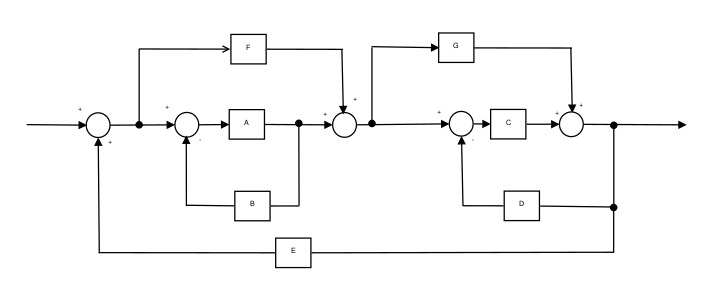
\includegraphics[scale=0.5]{./images/schema21.png}
	\end{figure}

	Possiamo utilizzare la \textbf{formula di Mason} per calcolare la funzione di trasferimento:
	\[
		H(s) = \frac{1}{\Delta}\sum_i P_i \Delta_i
	\]

	in cui:
	\begin{itemize}
		\item $\Delta$ = 1 - (tutti gli anelli) + (prodotto di tutti gli anelli che non si toccano \textit{a due a due}) - (prodotto di tutti gli anelli che non si toccano \textit{a tre a tre}) - ...
		\item $P_i$ = percorso i-esimo
		\item $\Delta_i$ = 1 - (tutti gli anelli che non toccano il percorso i-esimo)
	\end{itemize}
	Cominciamo individuando nello schema a blocchi tutti gli anelli e tutti i percorsi presenti: \\
	\textbf{anelli}: $A_1 = -AB$, \quad $A_2 = -CD$, \quad $A_3 = ACE$, \quad $A_4 = AGE$, \quad $A_5 = -FCE$, \quad $A_6 = FGE$\\
	\textbf{percorsi}: $P_1 = AC$ \quad $P_2 = FC$, \quad $P_3 = FG$, \quad $P_4 = AG$	\\ \\
	Calcoliamo il determinante $\Delta $: notiamo che abbiamo alcune coppie di anelli che non si toccano, ovvero AB e CD, AB e FCE, e infine AB e FGE. Per calcolare il determinante dobbiamo quindi aggiungere la somma dei prodotti di questi anelli:
	\[
		\Delta = 1-(-AB-CD+ACE+AGE+FCE+FGE)+(ABCD-ABFCE-ABFGE)
	\]
	\[
		= 1 + AB(1+CD-FCE-FGE)-E(AC+AG+FC+FG)+CD
	\]
	Calcoliamo ora i determinanti relativi ai singoli percorsi (ovvero $\Delta_1$, $\Delta_2$ ecc.). Notiamo che i percorsi $P_1$ e $P_4$ \textit{sono toccati da tutti gli anelli}, e quindi i rispettivi determinanti sono unitari.\\
	I percorsi $P_2$ e $P_3$, invece, \textit{non vengono toccati} dall'anello AB.\\
	$\Delta_1 = 1$\\
	$\Delta_2 = 1-AB$ \\
	$\Delta_3 = 1-AB$ \\
	$\Delta_4 = 1$ \\ \\
	Ora abbiamo tutti gli elementi per calcolare la funzione di trasferimento:
	\[
		H(s) = \frac{AC(1) + FC(1-AB) + FG(1-AB) + AG}{1 + AB(1+CD-FCE-FGE)-E(AC+AG+FC+FG)+CD}
	\]
	\newpage
	\paragraph*{Esercizio 2.2}
	Calcolare la funzione di trasferimento del seguente schema a blocchi:
	\begin{figure}[h!]
		\centering
		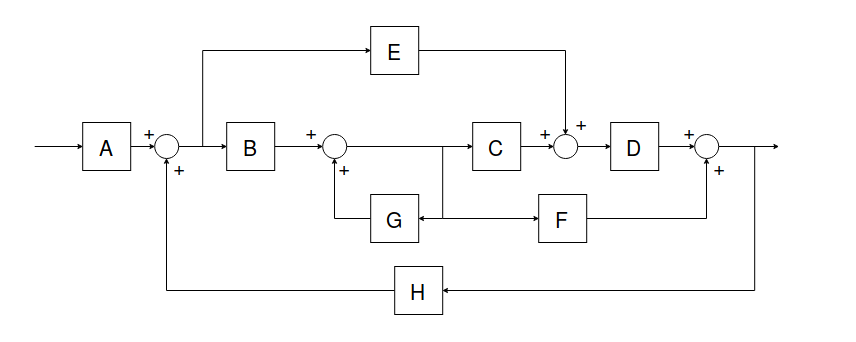
\includegraphics[scale=0.5]{./images/schema22.png}
	\end{figure}
    \\
	Individuiamo tutti gli anelli presenti nello schema a blocchi:\\
	$A_1 = G$, \quad $A_2 = BCDH$, \quad $A_3 = EDH$\\ \\
	I percorsi sono invece:\\
	$P_1 = ABCD$, \quad $P_2 = AED$, \quad $P_3 = ABF$\\ \\
	Utilizziamo quindi la formula di Mason per calcolare la funzione di trasferimento:
	\[
		H(s) = \frac{1}{\Delta}\sum_i P_i \Delta_i
	\]
	Calcoliamo $\Delta$: tutti gli anelli si toccano in qualche punto, quindi il determinante conterr\'a solo la sommatoria di tutti gli anelli:
	\[
		\Delta = 1 - (G + BCDH + EDH)
	\]
	Calcoliamo i determinanti relativi ai singoli percorsi, notando che il percorso $P_2$ non viene toccato dall'anello G:\\
	$\Delta_1 = 1$\\
	$\Delta_2 = 1-G$ \\
	$\Delta_3 = 1$ \\ \\
	Quindi la funzione di trasferimento risulta essere:
	\[
		H(s) = \frac{A(BCD + ED + BF)}{1 - G - DH(BC + E)}
	\]
	\newpage
 	\paragraph{Esercizio 2.3} Calcolare la funzione di trasferimento del seguente schema a blocchi:
 	\begin{figure}[h!]
 		\centering
 		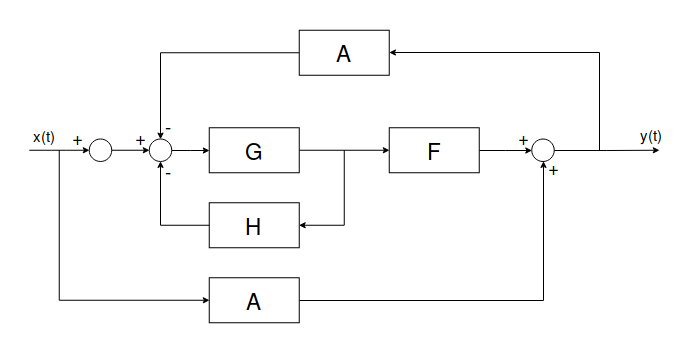
\includegraphics[scale=0.5]{./images/schema23.png}
 	\end{figure}

 	\hspace{-18px}\textbf{anelli}: $A_1 = -GH$ \quad $A_2 = -GFA$\\
 	\textbf{percorsi}: $P_1 = GF$ \quad $P_2 = A$ \\

 	\hspace{-18px}Calcoliamo $\Delta$:\\
 	$\Delta = 1 - (-GH-GFA) = 1 + GH + GFA$\\


 	\hspace{-18px}Calcoliamo i determinanti relativi ai vari percorsi:\\
 	$\Delta_1 = 1$\\
 	$\Delta_2 = 1-(-GH) = 1 + GH$\\

 	\hspace{-18px}Ora abbiamo tutti gli elementi per calcolare la formula di Mason:
 	\[
 		H(s) = \frac{1}{\Delta}\sum_i P_i \Delta_i = \frac{GF + A(1-GH)}{1+GH+GFA}
 	\]
	\newpage
	\paragraph*{Esercizio 2.4}
	Calcolare la funzione di trasferimento del seguente schema a blocchi:
	\begin{figure}[h!]
		\centering
		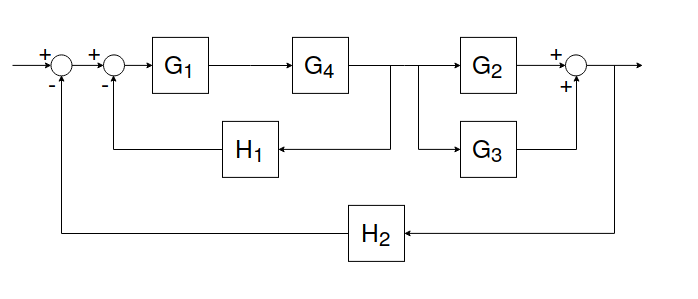
\includegraphics[scale=0.5]{./images/schema24.png}
	\end{figure}
	\\
	Gli anelli dello schema a blocchi sono:\\
	$A_1 = -G_1G_4H_1$,\quad$A_2 = -G_1G_4G_2H_2$\\ \\
	I percorsi sono invece:\\
	$P_1 = G_1G_4G_2$,\quad$P_2 = G_1G_4G_3$\\ \\
	\'E immediato notare che gli anelli presenti nello schema si toccano, e quindi il determinante sar\'a:
	\[
		\Delta = 1 - (-G_1G_4H_1 - G_1G_4G_2H_2) = 1 +G_1G_4H_1 + G_1G_4G_2H_2
	\]
	Inoltre, sia il percorso $P_1$ che il percorso $P_2$ toccano entrambi gli anelli in qualche punto, dunque i relativi determinanti sono semplicemente $\Delta_1 = 1$ e $\Delta_2 = 1$.\\
	Ora possiamo applicare la formula di Mason:
	\[
		H(s) = \frac{1}{\Delta}\sum_i P_i \Delta_i = \frac{1}{1 +G_1G_4H_1 + G_1G_4G_2H_2} \cdot \left(G_1G_4G_2 + G_1G_4G_3\right)
	\]
	Raccogliendo gli opportuni termini possiamo rendere la formula pi\'u leggibile:
	\[
		H(s) = \frac{G_1G_4(G_2+G_3)}{1+G_1G_4(H_1+G_2H_2)}
	\]
	\newpage
	\paragraph*{Esercizio 2.5 - appello del 13/09/2019} Calcolare la funzione di trasferimento del seguente sistema a blocchi:
	\begin{figure}[h!]
		\centering
		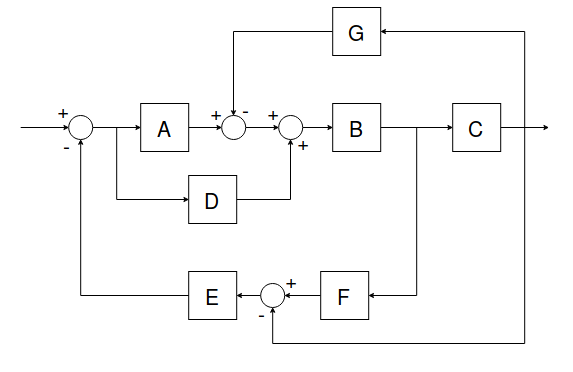
\includegraphics[scale=0.5]{./images/schema25.png}
	\end{figure}
	\\
	Iniziamo l'esercizio individuando tutti gli anelli e tutti i percorsi dello schema:
	\textbf{anelli:} $A_1 = -ABFE$,\quad$A_2 = ABCE$,\quad,$A_3=-BCG$,\quad$A_4 = -DBFE$\\
	\textbf{percorsi:} $P_1 = ABC$,\quad$P_2=DBC$\\ \\
	Tutti gli anelli si toccano in almeno un punto: unfatti, anche senza guardare lo schema a blocchi, notiamo che tutti passano dal blocco B.\\
	Quindi il determinante sar\'a:
	\[
		\Delta = 1-(-ABFE+ABCE-BCG-DBFE) = 1+ABFE-ABCE+BCG+DBFE
	\]
	Ora calcoliamo i determinanti $\Delta_1$ e $\Delta_2$ relativi ai singoli percorsi: notiamo che i percorsi passano tutti dal blocco B, e questo blocco \'e presente anche in tutti gli anelli. \\Quindi i determinanti dei percorsi saranno semplicemente $\Delta_1 = 1$ e $\Delta_2 = 1$.\\ \\
	Adesso abbiamo tutti gli elementi per utilizzare la formula di Mason e calcolare la funzione  di trasferimento dello schema a blocchi:
	\[
		H(s) = \frac{1}{\Delta}\sum_i P_i \Delta_i = \frac{ABC + DBC}{1+ABFE - ABCE + BCG + DBFE}
	\]
	\newpage
	\paragraph*{Esercizio 2.6} Calcolare la funzione di trasferimento del seguente schema a blocchi \textit{utilizzando l'algebra dei blocchi}:
	\begin{figure}[h!]
		\centering
		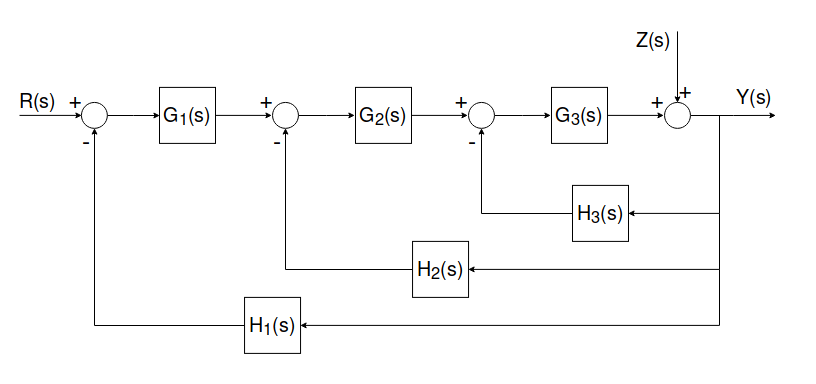
\includegraphics[scale=0.5]{./images/schema26.png}
	\end{figure}
	\\ In questo esercizio si chiede espressamente di non fare uso della formula di Mason, ma di calcolare la funzione di trasferimento operando le semplificazioni possibili tra i vari blocchi.\\
	Notiamo che in questo esercizio c'\'e una novit\'a: \underline{abbiamo due funzioni di ingresso, $R(s)$ e $Z(s)$}, anzich\'e una, come eravamo abituati.\\
	Tuttavia questo non cambia di molto il metodo di risoluzione dell'esercizio: possiamo spostare l'ingresso $Z(s)$ all'interno dello schema come fosse un qualsiasi altro blocco!
	\begin{itemize}
		\item cominciamo spostando la giunzione sommante in cui entra l'ingresso $Z(s)$ a monte del blocco $G_3(s)$:
		\begin{figure}[h!]
			\centering
			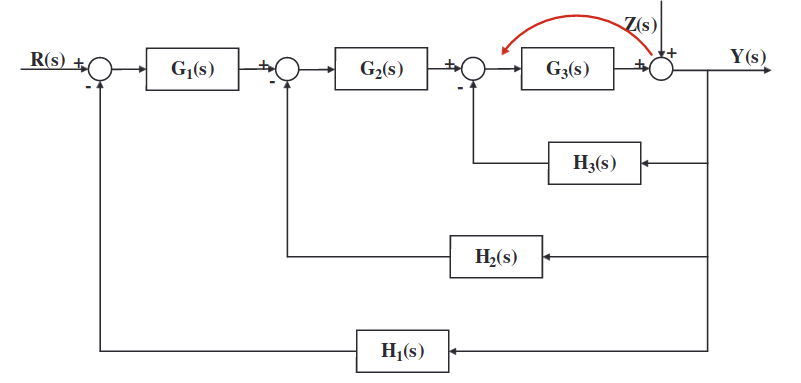
\includegraphics[scale=0.4]{./images/schema26_1.png}
		\end{figure}
		\\
		\item le giunzioni sommanti possono essere scambiate senza apportare altre modifiche, grazie alla propriet\`a commutativa dell'addizione:
		\begin{figure}[h!]
			\centering
			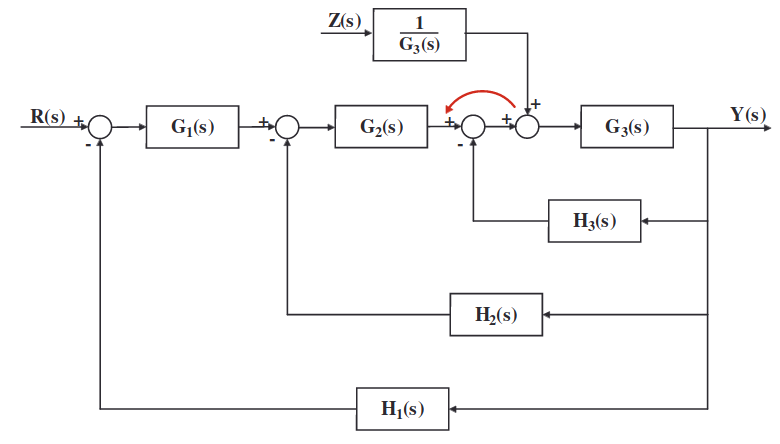
\includegraphics[scale=0.4]{./images/schema26_2.png}
		\end{figure}
		\item cos\`i facendo siamo riusciti a isolare un anello:
		\begin{figure}[h!]
			\centering
			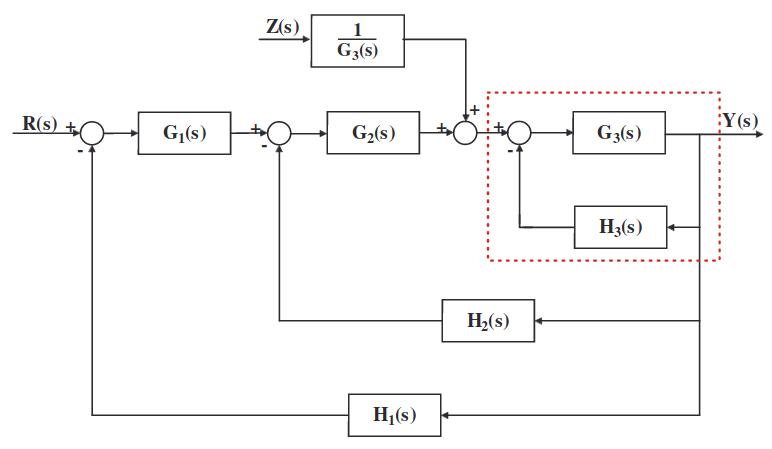
\includegraphics[scale=0.4]{./images/schema26_3.png}
		\end{figure}
		\item semplifichiamo i blocchi che appartengono all'anello e spostiamo ulteriormente il sommatore in cui entra l'ingresso $Z(s)$ a monte del blocco $G_2(s)$:
		\begin{figure}[h!]
			\centering
			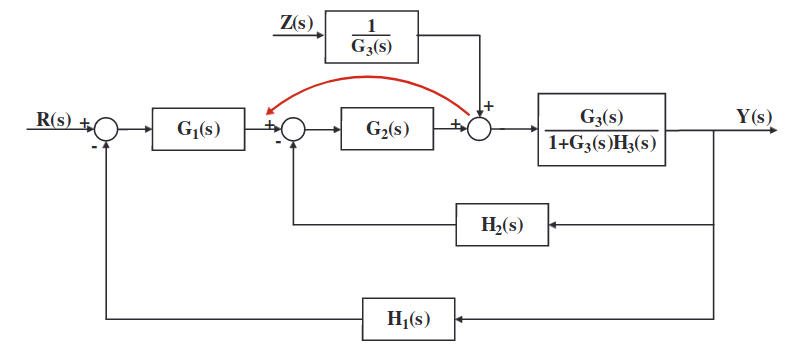
\includegraphics[scale=0.4]{./images/schema26_5.png}
		\end{figure}
		\\ \\ \\ \\ \\ \\ \\ \\ \\
		\item cos\`i facendo otteniamo due blocchi in serie e un anello:
		\begin{figure}[h!]
			\centering
			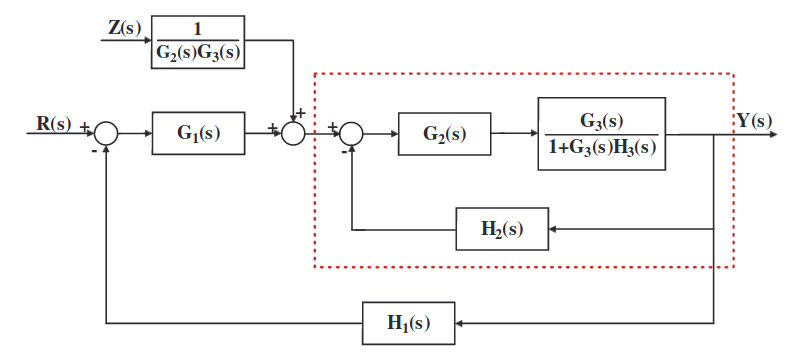
\includegraphics[scale=0.4]{./images/schema26_6.png}
		\end{figure}
		\item possiamo quindi semplificare tra loro questi blocchi ottenendo il seguente schema:
		\begin{figure}[h!]
			\centering
			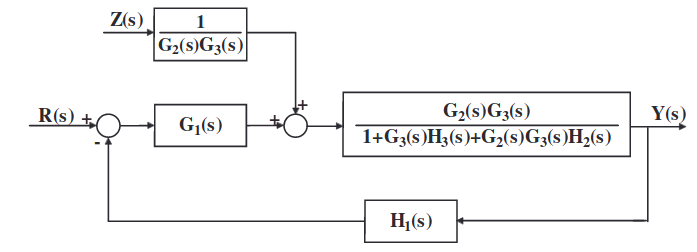
\includegraphics[scale=0.4]{./images/schema26_7.png}
		\end{figure}
		\item spostando la giunzione sommante di $Z(s)$ a monte del blocco $G_1(s)$ e del primo sommatore otteniamo nuovamente una serie e un anello, che possono essere semplicati come abbiamo fatto nel punto precedente:
		\begin{figure}[h!]
			\centering
			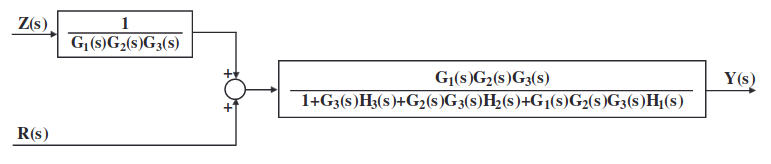
\includegraphics[scale=0.4]{./images/schema26_8.png}
		\end{figure}
		\\ \\
		\item come ultimo passaggio, spostiamo il blocco cos\`i ottenuto a monte della giunzione sommante e otteniamo il seguente schema:
		\begin{figure}[h!]
			\centering
			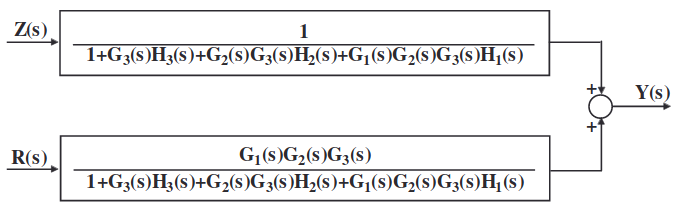
\includegraphics[scale=0.4]{./images/schema26_9.png}
		\end{figure}
	\end{itemize}
	Se chiamiamo la funzione scritta all'interno blocco superiore $A(s)$ e la funzione scritta nel blocco inferiore $B(s)$, la funzione di trasferimento $H(s)$ dello schema risulta essere:
	\[
		H(s) = A(s) + B(s)
	\]
	\newpage
	\paragraph*{Esercizio 2.7 - appello del 13/09/2019} Calcolare la funzione di trasferimento del seguente schema a blocchi:
	\begin{figure}[h!]
		\centering
		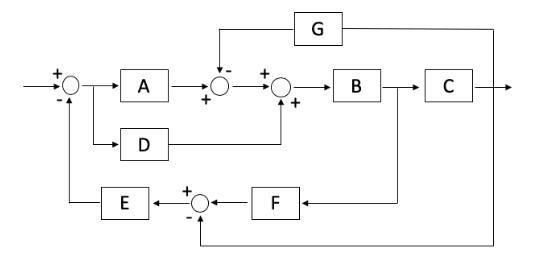
\includegraphics[scale=0.5]{./images/schema27.png}
	\end{figure}
	\\ Risolviamo questo esercizio utilizzando entrambi i metodi che conosciamo: prima con l'algebra dei blocchi, poi con la formula di Mason.\\ \\ \\
	\textbf{1^ metodo: algebra dei blocchi}
	\begin{itemize}
		\item invertiamo i nodi sommatori che si trovano tra il blocco A e il blocco B; inoltre sposto la diramazione a monte del blocco C:
		\begin{figure}[h!]
			\centering
			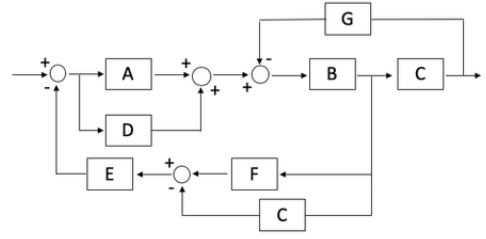
\includegraphics[scale=0.4]{./images/schema27_1.png}
		\end{figure}
		\item sposto l'altra diramazione a monte di C e risolvo i blocchi in parallelo A,D e F,C:
		\begin{figure}[h!]
			\centering
			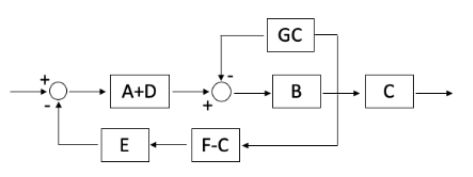
\includegraphics[scale=0.4]{./images/schema27_2.png}
		\end{figure}
		\item risolvo la serie nel ramo inferiore, composta dai blocchi E e F-C; inoltre risolvo la retroazione dei blocchi B e GC:
		\newpage
		\begin{figure}[h!]
			\centering
			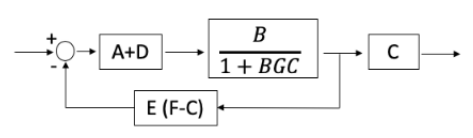
\includegraphics[scale=0.4]{./images/schema27_3.png}
		\end{figure}
		\item semplifico i blocchi in serie:
		\begin{figure}[h!]
			\centering
			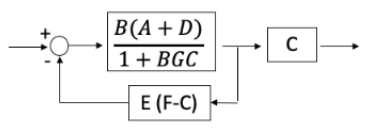
\includegraphics[scale=0.4]{./images/schema27_4.png}
		\end{figure}
		\item infine risolvo la retroazione, e ottengo:
		\begin{figure}[h!]
			\centering
			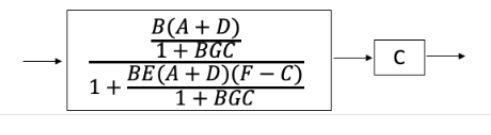
\includegraphics[scale=0.4]{./images/schema27_5.png}
		\end{figure}
	\end{itemize}
	Ora abbiamo solo due blocchi in serie, e sappiamo che questa configurazione si risolve moltiplicando i due blocchi.\\La funzione di trasferimento finale risulta quindi essere:
	\[
		H = \frac{BC(A+D)}{1+BGC+BEAF-BEAC+BEDF-BCED}
	\]
	\\ \\ \\
	\textbf{2^ metodo: formula di Mason}\\
	Individuiamo tutti i cammini del percorso:\\
	$P_1 = ABC$\\
	$P_2 = DBC$\\ \\
	Gli anelli presenti sono invece:\\
	$A_1 = -BCG$\\
	$A_2 = -ABFE$\\
	$A_3 = ABCE$\\
	$A_4 = BCED$\\
	$A_5 = -BFED$\\ \\
	Notiamo che tutti gli anelli si toccano in qualche punto: infatti tutti contengono passano dal blocco B!\\Il delta dello schema a blocchi sar\`a quindi:
	\[
		\Delta = 1-(-BCG-ABFE+ABCE+BCED-BFED) = 1+BCG+ABFE-ABCE-BCED+BFED
	\]
	Calcoliamo ora i delta relativi ai vari percorsi: \\
	$\Delta_1 = 1$\\
	$\Delta_2 = 1$\\
	Questo perch\`e tutti i percorsi e tutti gli anelli passano dal blocco B, quindi non esistono anelli che non toccano qualche percorso!\\
	Applicando la formula di Mason, ricaviamo che la trasmittanza totale dello schema \`e uguale a quella calcolata con il metodo precedente:
	\[
		H = \frac{1}{\Delta}\sum_i P_i\Delta_i
	\]
	\[
		H = \frac{1}{1+BCG+ABFE-ABCE-BCED+BFED}\cdot ABC(1) + DBC(1)
	\]
	\[
		H = \frac{BC(A+D)}{1+BGC+BEAF-BEAC+BEDF-BCED}
	\]
	\newpage
	\section*{Sistemi LTI a tempo discreto}
	\paragraph*{Esercizio 3.1 - appello del 01/07/2019, versione A}
	Dato il sistema LTI causale a tempo discreto descritto dalla seguente equazione alla differenze:
	\[
		\begin{cases}
		v(k) - v(k-1) -\frac{3}{4}v(k-2) = -\frac{5}{2}u(k) - \frac{3}{4}u(k-1)\\
		v(-1) = 2\\
		v(-2) = -1\\
		u(k) = \left(-\frac{1}{2}\right)^k\delta_{-1}(k)
		\end{cases}
	\]
	\begin{enumerate}
	\item Calcolare la risposta libera nel tempo (esclusivamente nel tempo!)
	\item Si discuta la stabilit\`a asintotica e la stabilit\`a BIBO
	\item Calcolare la risposta impulsiva del sistema utilizzando l'antitrasformata Zeta
	\item Calcolare la risposta totale del sistema utilizzando l'antitrasformata Zeta
	\end{enumerate}
	---------------------------------------------------------------------------------------------------------------------------\\
	\begin{enumerate}
	\item Scriviamo innanzitutto l'equazione caratteristica del sistema e calcoliamo le sue radici:
	\[
		z^2-z-\frac{3}{4} = 0
		\Longleftrightarrow
		4z^2-4z-3 = 0
	\]
	Le radici di questa equazione sono $z_1 = \frac{3}{2}$ e $z_2 = -\frac{1}{2}$.\\
	L'espressione dell'evoluzione libera sar\`a dunque nella forma:
	\[
		v_l(k) = c_1\left(\frac{3}{2}\right)^k + c_2\left(-\frac{1}{2}\right)^k
	\]
	Per trovare il valore dei coefficienti $c_1$ e $c_2$ devo semplicemente imporre le condizioni iniziali:
	\[
		\begin{cases}
		v(-1) = 2 = c_1\left(\frac{3}{2}\right)^{-1} + c_2\left(-\frac{1}{2}\right)^{-1}\\
		v(-2) = -1 = c_1\left(\frac{3}{2}\right)^{-2} + c_2\left(-\frac{1}{2}\right)^{-2}
		\end{cases}
		\Longrightarrow
		\begin{cases}
		c_1 = 3 + 3c_2\\
		(3+3c_2)\left(\frac{4}{9}\right) + c_2(4) = -1
		\end{cases}
	\]
	Risolvendo queste equazioni si trova che $c_1 = \frac{27}{16}$ e $c_2 = -\frac{7}{16}$.\\
	Possiamo quindi scrivere l'espressione definitiva dell'evoluzione libera:
	\[
		v_l(k) = \frac{27}{16}\left(\frac{3}{2}\right)^k -\frac{7}{16}\left(-\frac{1}{2}\right))^k
	\]
	\item Il sistema è \textbf{asintoticamente stabile} se e solo se tutte le radici caratteristiche sono in modulo minori di 1, quindi $|z_1| < 1$, ... , $|z_n| < 1$\\
	Nel nostro caso per\`o, notiamo subito che $|z_1| = |\frac{3}{2}| > 1$, e dunque concludiamo che il sistema \textit{non è asintoticamente stabile}.\\
	Verifichiamo ora la stabilit\`a BIBO analizzando la funzione di trasferimento del sistema: il sistema \`e BIBO stabile se e solo se tutti i poli che causano l'instabilit\`a asintotica (nel nostro caso, $z_1$) si semplificano.
	\[
		H(z) = \frac{-\frac{5}{2}z^2 - \frac{3}{4}z}{\left(z-\frac{3}{2}\right) \left(z+\frac{1}{2}\right)}
	\]
	Ma il polo $z_1$ non viene semplificato, dunque il sistema \textit{non \`e BIBO stabile}.
	\item La risposta impulsiva del sistema si ricava eseguendo l'antitrasformata Zeta della funzione di trasferimento:
	\[
		H(z) = \frac{z\left(-\frac{5}{2}z - \frac{3}{4}\right)}{\left(z-\frac{3}{2}\right)\left(z+\frac{1}{2}\right)}
	\]
	L'antitrasformata si ottiene seguendo questi passaggi:
	\begin{itemize}
		\item Divido $H(z)$ per z:
		\[
			\frac{H(z)}{z} = \frac{-\frac{5}{2}z - \frac{3}{4}}{\left(z-\frac{3}{2}\right)\left(z+\frac{1}{2}\right)}
		\]
		\item Scompongo in fratti semplici:
		\[
			\frac{H(z)}{z} = \frac{A}{\left(z-\frac{3}{2}\right)} + \frac{B}{\left(z+\frac{1}{2}\right)}
		\]
		Calcolo i coefficienti A e B:\\ \\
		$A = \left(z-\frac{3}{2}\right)\frac{-\frac{5}{2}z - \frac{3}{4}}{\left(z-\frac{3}{2}\right)\left(z+\frac{1}{2}\right)}\Biggl\vert_{s=\frac{3}{2}} = -\frac{9}{4}$\\
		$B = \left(z+\frac{1}{2}\right)\frac{-\frac{5}{2}z - \frac{3}{4}}{\left(z-\frac{3}{2}\right)\left(z+\frac{1}{2}\right)}\Biggl\vert_{s=-\frac{1}{2}} = -\frac{1}{4}$\\
		\\ \\
		Da cui ricaviamo l'espressione scomposta:
		\[
			\frac{H(z)}{z} = -\frac{9}{4}\Biggl(\frac{1}{z-\frac{3}{2}}\Biggr) - \frac{1}{4}\Biggl(\frac{1}{z+\frac{1}{2}}\Biggr)
		\]
		\item Moltiplico per z:
		\[
			H(z) = -\frac{9}{4}\Biggl(\frac{z}{z-\frac{3}{2}}\Biggr) - \frac{1}{4}\Biggl(\frac{z}{z+\frac{1}{2}}\Biggr)
		\]
		\item Ora posso ricavare la funzione antitrasformata, che è esattamente la risposta impulsiva che cercavamo:
		\[
			h(k) = \Bigl[\frac{9}{4}\left(\frac{3}{2}\right)^k - \frac{1}{4}\left(-\frac{1}{2}\right)^k\Bigr]\delta_{-1}(k)
		\]
	\end{itemize}
	\item Applico la trasformata Zeta all'ingresso e all'uscita:
	\[
		z^0V(z) - [z^{-1}V(z) + v(-1)z^0] - \frac{3}{4}[z^{-2}V(z) + v(-2)z^0 + v(-1)z^{-1}] = -\frac{5}{2}z^0U(z)-\frac{3}{4}z^{-1}U(z)
	\]
	\[
		V(z) - \frac{1}{z}V(z) - 2 - \frac{3}{4}\left(\frac{1}{z^2}V(z)-1+2\frac{1}{z}\right) = -\frac{5}{2}U(z) - \frac{3}{4z}U(z)
	\]
	\\
	Raccogliendo V(z) e U(z) si ottiene:
	\[
		V(z) = U(z)\frac{-\frac{5}{2}z^2-\frac{3}{4}z}{z^2-z-\frac{3}{4}} + \frac{\frac{5}{4}z^2-\frac{3}{2}z}{z^2-z-\frac{3}{4}}
	\]
	Dato che $u(k) = \left(-\frac{1}{2}\right)^k\delta_{-1}(k)$, ricaviamo facilmente che $U(z) = \mathcal{Z}[u(k)] = \frac{z}{z+\frac{1}{2}}$\\ \\
	E quindi l'espressione finale di $V(z)$ sar\`a:
	\[
		V(z) = \frac{z\left(-\frac{5}{2}z^2-\frac{7}{8}z-\frac{3}{2}\right)}{\left(z+\frac{1}{2}\right)^2\left(z-\frac{3}{2})\right)}
	\]
	Ora applico l'algoritmo descritto al punto precedente per calcolare l'antitrasformata Zeta di $V(z)$ con il metodo dei fratti semplici:
	\[
		\frac{V(z)}{z} = \frac{A}{\left(z+\frac{1}{2}\right)} + \frac{B}{\left(z+\frac{1}{2}\right)^2} + \frac{C}{\left(z-\frac{3}{2}\right)}
	\]
	\textbf{Attenzione!} Il polo $z = -\frac{1}{2}$ ha molteplicit\`a 2, dunque il coefficiente A dovr\`a essere calcolato con la derivata:\\ \\
	$A=\frac{d}{dz}\left( \left(z+\frac{1}{2}\right)^2\frac{-\frac{5}{4}z^2-\frac{7}{8}z-\frac{3}{2}}{\left(z+\frac{1}{2}\right)^2\left(z-\frac{3}{2}\right)}\right)\Bigl\vert_{z=-\frac{1}{2}} = -\frac{3}{16}$	\\ \\
	$B=\left(\left(z+\frac{1}{2}\right)^2\frac{-\frac{5}{4}z^2-\frac{7}{8}z-\frac{3}{2}}{\left(z+\frac{1}{2}\right)^2\left(z-\frac{3}{2}\right)}\right)\Bigl\vert_{z=-\frac{1}{2}} = -\frac{1}{2}$ \\ \\
	$C=\left(\left(z-\frac{3}{2}\right)^2\frac{-\frac{5}{4}z^2-\frac{7}{8}z-\frac{3}{2}}{\left(z+\frac{1}{2}\right)^2\left(z-\frac{3}{2}\right)}\right)\Bigl\vert_{z=\frac{3}{2}} = -\frac{27}{64}$ \\ \\
	Otteniamo quindi l'espressione scomposta di V(z):
	\[
		V(z) = -\frac{3}{16}
		\left(\frac{z}{z+\frac{1}{2}}\right)
		+ \frac{1}{2}\left(\frac{z}{(z+\frac{1}{2})^2}\right)
		+ \frac{27}{64}\left(\frac{z}{z-\frac{3}{2}}\right)
	\]
	Da cui ricaviamo facilmente l'antitrasformata:
	\[
		v(k) = \left[\frac{3}{16}\left(-\frac{1}{2}\right)^k + \frac{1}{2}k\left(-\frac{1}{2}\right)^k + \frac{27}{64}\left(\frac{3}{2}\right)^k\right]\delta_{-1}(t)
	\]
	Notare che il secondo termine $\left(-\frac{1}{2}\right)^k$ \`e moltiplicato per un fattore k: questo \`e sempre dovuto al fatto che quel polo ha molteplicit\`a 2.
	\end{enumerate}
	\newpage
	\paragraph*{Esercizio 3.2 - appello del 17/07/2017} Dato il seguente sistema LTI a tempo discreto
	\[
		\begin{cases}
			9v(k) + 6v(k-1) + v(k-2) = 3u(k) + u(k-1) \\
			v(-1) = 1 \\
			v(-2) = 1 \\
			u(t) = \delta_{-1}(k)
		\end{cases}
	\]

	\begin{enumerate}
		\item Calcolare l'evoluzione libera del sistema nel dominio del tempo
		\item Discutere la stabilit\`a del sistema
		\item Calcolare la risposta impulsiva nel dominio del tempo
		\item Calcolare la risposta totale con l'antitrasformata Zeta

	\end{enumerate}
	-------------------------------------------------------------------------------------------------------------------------\\
	\begin{enumerate}
		\item Cominciamo calcolando le radici dell'equazione caratteristica:
		\[
			9z^2 + 6z + 1 = 0
			\Rightarrow
			z_{1,2} = -\frac{1}{3}
		\]
		Notare che la molteplicit\`a algebrica della radice è 2 ($\mu = 2$)! \\
		L'espressione dell'evoluzione libera sar\`a dunque nella forma:
		\[
			v_l(k) = c_1\left(-\frac{1}{3}\right)^k + kc_2\left(-\frac{1}{3}\right)^k
		\]
		Impongo le condizioni iniziali del sistema per ricavare i coefficienti $c_1$ e $c_2$:
		\[
			\begin{cases}
				v(-1) = 1 = c_1\left(-\frac{1}{3}\right)^{-1} + (-1)c_2\left(-\frac{1}{3}\right)^{-1} \\
				v(-2) = 1 = c_1\left(-\frac{1}{3}\right)^{-2} + (-2)c_2\left(-\frac{1}{3}\right)^{-2} \\
			\end{cases}
			\Rightarrow
			\begin{cases}
				c_1 = -\frac{7}{9}\\
				c_2 = \frac{10}{9}\\
			\end{cases}
		\]
		Quindi l'espressione finale dell'evoluzione libera \`e:
		\[
			v_l(k) = -\frac{7}{9}\left(-\frac{1}{3}\right)^k + k\frac{10}{9}\left(-\frac{1}{3}\right)^k
		\]
		\item Il sistema è \textbf{asintoticamente stabile} se $|z_1|$, $|z_2|$, ... , $|z_n| < 1$. \\
		Nel nostro caso, $|-\frac{1}{3}| = \frac{1}{3} < 1$, quindi il sistema è asintoticamente stabile.\\
		La stabilit\`a asintotica implica la BIBO stabilit\`a, quindi il nostro sistema \`e anche BIBO stabile.
		\item L'espressione della risposta impulsiva \`e nella forma:
		\[
			h(k) = \left[d_1\left(-\frac{1}{3}\right)^k + kd_2\left(-\frac{1}{3}\right)^k\right]\delta_{-1}(k)
		\]
		Per ricavare i coefficienti $d_1$ e $d_2$, devo sostituire nell'espressione originale del sistema $v(k)$ con $h(k)$, e $u(k)$ con $\delta(k)$.\\
		Per capirne il motivo, \`e sufficiente pensare al significato stesso della \textit{risposta impulsiva}: essa è definita come l'uscita del sistema in risposta a un impulso unitario!\\ \\
		Dopo aver effettuato la sostituzione, troviamo dunque la seguente espressione:
		\[
			9h(k) + 6h(k-1) + h(k-2) = 3\delta(k) + \delta (k-1)
		\]
		\fbox {\textit{k = 0}} : $9h(0) + 6h(-1) + h(-2) = 3\delta(0) + \delta(-1)$
		\medskip
		\\
		Sappiamo che la risposta impulsiva è nulla per valori negativi di k e che l'impulso\\ è non nullo solo nell'origine, quindi per k = 0. Quindi alla fine resta:\\
		\medspace
		$9h(0) = 3$ \hspace*{10px} $\Rightarrow$ \hspace*{10px} $h(0) = \frac{1}{3}$ \\ \\
		\fbox {\textit{k = 1}} : $9h(1) + 6h(0) + h(-1) = 3\delta(1) + \delta(0)$
		\medskip
		\\
		Da cui si ricava facilmente che $h(1) = -\frac{1}{9}$. \\ \\
		Ora ricaviamo i coefficienti $d_1$ e $d_2$ impostando il sistema seguente:\\
		\[
			\begin{cases}
				h(0) = \frac{1}{3} = \left[d_1 + 0\cdot d_2\right] \delta_{-1}(0) \\
				h(1) = -\frac{1}{9} = \left[-\frac{1}{3}d_1 + -\frac{1}{3} d_2\right] \delta_{-1}(1) \\
			\end{cases}
		\]
		Da cui si ricava che $d_1 = \frac{1}{3}$ e $d_2 = 0$.\\ \\
		Possiamo quindi scrivere l'espressione finale della risposta impulsiva:
		\[
			h(k) = \frac{1}{3}\left(-\frac{1}{3}\right)^k\delta_{-1}(k)
		\]
		\item Calcoliamo la risposta totale del sistema applicando la trasformata Zeta all'ingresso e all'uscita:
		\[
			\mathcal{Z}\left[9v(k) + 6v(k-1) + v(k-2)\right] = \mathcal{Z}\left[3u(k) + u(k-1)\right]
		\]
		\[
			9z^0V(z) + 6\left(z^{-1}V(z) + v(-1) \cdot z^0\right) + z^{-2} V(z) + v(-2)z^0 + v(-1)z^{-1} = 3z^0U(z) + z^{-1}U(z)
		\]
		Eseguendo gli opportuni calcoli, e isolando V(z) otteniamo l'espressione:
		\[
			V(z) = U(z) \frac{3+\frac{1}{z}}{9+\frac{6}{z} + \frac{1}{z^2}} - \frac{7 + \frac{1}{z}}{9 + \frac{6}{z} + \frac{1}{z^2}}
		\]
		Moltiplicando numeratore e denominatore per $\frac{1}{z^2}$, e tenendo conto che $U(z) = \mathcal{Z}\left[u(k)\right] = \frac{1}{z}$:
		\[
			V(z) = \frac{1}{z} \cdot \frac{3z^2+z}{\left(z+\frac{1}{3}\right)^2} - \frac{7 + \frac{1}{z}}{\left(z+\frac{1}{3}\right)^2}
		\]
		I passaggi da effettuare per ricavare l'antitrasformata della nostra funzione, e dunque l'espressione della risposta totale nel tempo, sono:
		\begin{itemize}
			\item dividere $V(z)$ per $z$:
				\[
					\frac{V(z)}{z} = \frac{-7z^2+2z+1}{z\left(z+\frac{1}{3}\right)^2}
				\]
			\item scomporre l'espressione trovata in fratti semplici:
				\[
					\frac{V(z)}{z} = \frac{A}{z} + \frac{B}{z\left(z+\frac{1}{3}\right)} + \frac{C}{z\left(z+\frac{1}{3}\right)^2}
				\]
				Notare che abbiamo il coefficiente B deve essere calcolato con la derivata, perché $z = -\frac{1}{3}$ \`e un polo di molteplicit\`a 2!\\
				$A = z \cdot \frac{-7z^2+2z+1}{z\left(z+\frac{1}{3}\right)^2} \Bigl\lvert_{z = 0} = 9$ \\ \\
				$B = \frac{d}{dz}\left(\left( z + \frac{1}{3}\right)^2 \cdot \frac{-7z^2+2z+1}{z\left(z+\frac{1}{3}\right)^2} \right)\Bigl\lvert_{z = -\frac{1}{3}}=-2$\\ \\
				$C = \left(z + \frac{1}{3}\right)^2 \cdot \frac{-7z^2+2z+1}{z\left(z+\frac{1}{3}\right)^2} \Bigl\lvert_{z = -\frac{1}{3}} = \frac{4}{3}$\\ \\
				Quindi
				\[
					\frac{V(z)}{z} = 9\left(\frac{1}{z}\right) - 2\left(\frac{1}{z+\frac{1}{3}}\right) +
					\frac{4}{3}\left(\frac{1}{\left(z + \frac{1}{3}\right)^2}\right)
				\]
			\item moltiplicare il risultato per z e antitrasformare:
			\[
				V(z) = 9 - 2\frac{z}{z+\frac{1}{3}} + \frac{4}{3}\frac{z}{\left(z+\frac{1}{3}\right)^2}
			\]
			Da cui il risultato:
			\[
				v(k) = 9\delta (k) + \left[-2\left(-\frac{1}{3}\right)^k + \frac{4}{3}k\left(-\frac{1}{3}\right)^k\right]\delta_{-1}(k)
			\]
		\end{itemize}
	\end{enumerate}
	\newpage
	\paragraph*{Esercizio 3.3 - parziale del 13/06/2019} Dato il seguente sistema LTI a tempo discreto:
	\[
		\begin{cases}
		v(k) + \frac{5}{14}v(k-1) -\frac{1}{14}v(k-2) = u(k) + 7u(k-2) \\
		v(-1) = 1 \\
		v(-2) = -2 \\
		u(t) = \left(-\frac{1}{2}\right)^k\delta_{-1}(k)
		\end{cases}
	\]
	\begin{enumerate}
		\item Calcolare l'evoluzione libera del sistema nel dominio del tempo
		\item Discutere la stabilit\`a del sistema
		\item Calcolare la risposta impulsiva con l'antitrasformata Zeta
		\item Calcolare la risposta totale con l'antitrasformata Zeta
	\end{enumerate}
	---------------------------------------------------------------------------------------------------------------------------\\
	\begin{enumerate}
		\item Scriviamo l'equazione caratteristica del sistema e calcoliamone le radici:
		\[
			z^2 + \frac{5}{14}z -\frac{1}{14} = 0
		\]
		Che ha come soluzioni $z_1 = -\frac{1}{2}$, $z_2 = \frac{1}{7}$.\\
		Quindi
		\[
			v_l(k) = c_1\left(-\frac{1}{2}\right)^k + c_2\left(\frac{1}{7}\right)^k
		\]
		Impongo le condizioni iniziali:
		\[
			\begin{cases}
				v(-1) = 1 = 7c_1 - 2c_2\\
				v(-2) = -2 = 49c_1 + 4c_2\\
			\end{cases}
			\Rightarrow
			\begin{cases}
				c_1 = 0\\
				c_2 = -\frac{1}{2}
			\end{cases}
		\]
		Quindi l'espressione definitiva dell'evoluzione libera sar\`a
		\[
			v_l(k) = -\frac{1}{2}\left(-\frac{1}{2}\right)^k
		\]
		\item Notiamo subito che $|z_1| = \frac{1}{2} < 1$ e $|z_2| = \frac{1}{7} < 1$ : entrambe le radici si trovano all'interno del cerchio unitario, quindi possiamo concludere che il sistema \`e \textbf{asintoticamente stabile} e, di conseguenza, \`e anche \textbf{BIBO stabile}.
		\item La risposta impulsiva si ricava facendo l'antitrasformata Zeta della funzione di trasferimento H(z):
		\[
			H(z) = \frac{7z^2-1}{\left(z - \frac{1}{7}\right) \left(z + \frac{1}{2}\right)}
		\]
		Dividendo per z si ottiene:
		\[
				\frac{H(z)}{z} = \frac{7z^2-1}{z\left(z - \frac{1}{7}\right) \left(z + \frac{1}{2}\right)}
		\]
		Scomponiamo quindi in fratti semplici:
		\[
			\frac{H(z)}{z} = \frac{A}{z} + \frac{B}{ \left(z + \frac{1}{2}\right)} + \frac{C}{\left(z - \frac{1}{7}\right)}
		\]
		$A = z \cdot \frac{7z^2-1}{z\left(z - \frac{1}{7}\right) \left(z + \frac{1}{2}\right)}\Bigl\lvert_{z = 0} = 14$\\ \\
		$B = \left( z + \frac{1}{2}\right) \cdot \frac{7z^2-1}{z\left(z - \frac{1}{7}\right) \left(z + \frac{1}{2}\right)} \Bigl\lvert_{z = -\frac{1}{2}} = \frac{7}{3}$ \\ \\
		$C = \left( z - \frac{1}{7}\right) \cdot \frac{7z^2-1}{z\left(z - \frac{1}{7}\right) \left(z + \frac{1}{2}\right)} \Bigl\lvert_{z = \frac{1}{7}} = -\frac{28}{3}$ \\ \\
		Quindi l'espressione di $\frac{H(z)}{z}$ si pu\`o riscrivere, scomposta, come:
		\[
			\frac{H(z)}{z} = \frac{14}{z} - \frac{28}{3} \frac{1}{\left(z-\frac{1}{7}\right)} + \frac{7}{3}\frac{1}{\left(z+\frac{1}{2}\right)}
		\]
		Moltiplico per z e antitrasformo, ottenendo cos\`i l'espressione finale della risposta impulsiva:
		\[
			h(t) = 14\delta(k) - \left[ \frac{28}{3}\left(\frac{1}{7}\right)^k\delta(k-1) + \frac{7}{3}\left(-\frac{1}{2}\right)^k\delta(k-2)\right]\delta_{-1}(k)
		\]
		\item Per calcolare la risposta totale del sistema, applico la trasformata Zeta all'ingresso e all'uscita:
		\[
			\mathcal{Z}\left[ v(k) + \frac{5}{14}v(k-1) -\frac{1}{14}v(k-2) \right] = \mathcal{Z} \left[ u(k) + 7u(k-2) \right]
		\]
		Da cui otteniamo:
		\[
			z^0V(z) + \frac{5}{14}\left( z^{-1}V(z) + v(-1)z^0 \right) - \frac{1}{14}\left( z^{-2} V(z) + v(-2) z^0 + v(-1)z^{-1}\right) = 7z^0U(z) - z^{-2}U(z)
		\]
		Moltiplico a sinistra e a destra per $z^2$ e raccolgo V(z) e U(z): \\ \\
		$V(z)(z^2 + \frac{5}{14}z - \frac{1}{14}) + \frac{5}{14}z^2 + \frac{2}{14}z^2 - \frac{1}{14}z = U(z)(7z^2-1)$ \\ \\
		$V(z) = \frac{7z^2-1}{\left(z-\frac{1}{7}\right) \left( z + \frac{1}{2} \right)}U(z) + \frac{-\frac{1}{2}z^2 + \frac{1}{14}z}{\left(z-\frac{1}{7}\right) \left( z + \frac{1}{2} \right)} $ \\ \\ \\
		Dato che $	u(t) = \left(-\frac{1}{2}\right)^k\delta_{-1}(k) $, si ricava facilmente che $U(z) = \frac{z}{z + \frac{1}{2}}$, e quindi l'espressione che abbiamo trovato si riscrive come:\\ \\
		$ V(z)= \frac{7z^2-1}{\left(z-\frac{1}{7}\right) \left( z + \frac{1}{2} \right)} \cdot \frac{z}{z + \frac{1}{2}} + \frac{-\frac{1}{2}z^2 + \frac{1}{14}z}{\left(z-\frac{1}{7}\right) \left( z + \frac{1}{2} \right)} = \frac{z\left(\frac{13}{2}z^2 - \frac{5}{28}z - \frac{27}{28}\right)}{\left(z-\frac{1}{7}\right) \left(z + \frac{1}{2}\right)^2} $ \\ \\ \\
		Divido per z e scompongo in fratti semplici:
		$\frac{V(z)}{z} = \frac{A}{\left(z-\frac{1}{7}\right)} + \frac{B}{ \left( z + \frac{1}{2} \right)^2} + \frac{C}{\left( z + \frac{1}{2} \right)}$ \\ \\ \\
		Ora, per ricavare il valore dei coefficienti A, B e C \`e sufficiente applicare il solito metodo dei fratti semplici, prestando attenzione al fatto che il polo $z = -\frac{1}{2}$ ha molteplicità 2, e C si calcola con la derivata.
		Si dovrebbe ottenere il seguente risultato:\\ \\
		$A = \frac{56}{27}$ \\ \\
		$B = \frac{343}{42}$ \\ \\
		$C = -\frac{137}{49}$ \\ \\ \\
		Ora possiamo facilmente antitrasformare $\frac{V(z)}{z}$ per ottenere l'espressione della risposta totale:
		\[
			v(t) = \left[ \frac{56}{27}\left(\frac{1}{7}\right)^k + \frac{343}{42}k\left(-\frac{1}{2}\right)^k - \frac{137}{49}\left(-\frac{1}{2}\right)^k\right]\delta_{-1}(k)
		\]
		\end{enumerate}
		\newpage
		\paragraph*{Esercizio 3.4 - esame del 16/06/2017} Si consideri il seguente sistema LTI a tempo discreto:
		\[
			\begin{cases}
			v(k) - \frac{1}{9}v(k-2) = 2u(k) + u(k-1) + \frac{1}{2}u(k-2)\\
			v(-1) = 0\\
			v(-2) = 1\\
			u(t) = \delta_{-1}(k)
			\end{cases}
		\]
		\begin{enumerate}
			\item Calcolare la risposta libera nel tempo
			\item Discutere la stabilit\`a del sistema
			\item Calcolare l'evoluzione forzata con l'antitrasformata Zeta
			\item Calcolare la risposta totale con l'antitrasformata Zeta
		\end{enumerate}
		-------------------------------------------------------------------------------------------------------------------\\
		\begin{enumerate}
			\item L'equazione caratteristica del sistema è
			\[
				z^2 - \frac{1}{9} = 0
			\]
			le cui radici sono $z_1 = \frac{1}{3}$, di molteplicit\`a $\mu_1 = 1$, e $z_2 = -\frac{1}{3}$, di molteplicit\`a $\mu_2 = 1$.
			Quindi l'espressione dell'evoluzione libera sar\`a del tipo
			\[
				v_l(k) = c_1\left(\frac{1}{3}\right)^k + c_2\left(-\frac{1}{3}\right)^k
			\]
			Ricaviamo i coefficienti $c_1$ e $c_2$ nel solito modo, imponendo le condizioni iniziali che ci vengono date e mettendo le equazioni a sistema:
			\[
				\begin{cases}
				v(-1) = 0 = c_1\left(\frac{1}{3}\right)^{-1} + c_2\left(-\frac{1}{3}\right)^{-1} \\
				v(-2) = 1 = c_1\left(\frac{1}{3}\right)^{-2} + c_2\left(-\frac{1}{3}\right)^{-2} \\
				\end{cases}
				\Rightarrow
				c_1 = c_2 = \frac{1}{18}
			\]
			Dunque l'espressione finale dell'evoluzione libera \`e:
			\[
				v_l(k) = \frac{1}{18}\left(\frac{1}{3}\right)^k + \frac{1}{18}\left(-\frac{1}{3}\right)^k
			\]
			\item $|z_1| = \left|\frac{1}{3}\right| < 1$ e $|z_2| = \left|-\frac{1}{3}\right| = \frac{1}{3} < 1 $, quindi il sistema \`e asintoticamente stabile e, di conseguenza, è anche BIBO stabile.
			\item Nel dominio del tempo, l'evoluzione forzata è data dalla \textit{convoluzione} tra la risposta impulsiva $h(k)$ e l'ingresso $u(k)$.\\Nel dominio della trasformata Zeta, la convoluzione corrisponde a una moltiplicazione, e quindi la trasformata zeta dell'evoluzione forzata si ricava \textit{moltiplicando} la trasformata della risposta impulsiva per la trasformata dell'ingresso:\\
			\[
				v_f(k) = h(k) * u(k)
				\Rightarrow
				\mathcal{Z}[v_f] = \mathcal{Z}[h(k) * u(k)]
				\Rightarrow
				V_f(z) = H(z) \cdot U(z)
			\]
			(si veda p. 205 del libro).\\ \\
			$H(z)$ non \`e altro che la funzione di trasferimento, ovvero il rapporto tra gli ingressi e le uscite:
			\[
				H(z) = \frac{2z^2 + z + \frac{1}{2}}{z^2 - \frac{1}{9}}
			\]
			$U(z)$, invece, si ricava applicando normalmente la trasformata Zeta all'ingresso dato:
			\[
				U(z) = \mathcal{Z}[\delta_{-1}(k)] = \frac{z}{z-1}
			\]
			A questo punto abbiamo tutti gli elementi per ricavare l'espressione di $V_f$:
			\[
				V_f(z) = \frac{2z^2 + z + \frac{1}{2}}{z^2 - \frac{1}{9}} \cdot \frac{z}{z-1} = \frac{\left(2z^2 + z + \frac{1}{2}\right)z}{\left(z-\frac{1}{3}\right)\left(z+\frac{1}{3}\right)\left(z-1\right)}
			\]
			Divido per z:
			\[
				\frac{V_f(z)}{z} = \frac{\left(2z^2 + z + \frac{1}{2}\right)z}{z\left(z-\frac{1}{3}\right)\left(z+\frac{1}{3}\right)\left(z-1\right)}
			\]
			Scompongo in fratti semplici:
			\[
				\frac{V_f(z)}{z} = \frac{A}{z} + \frac{B}{z-\frac{1}{3}} + \frac{C}{z+\frac{1}{3}} + \frac{D}{z-1}
			\]
			$A = \frac{\left(2z^2 + z + \frac{1}{2}\right)z}{\left(z-\frac{1}{3}\right)\left(z+\frac{1}{3}\right)\left(z-1\right)}\Bigl\lvert_{z=0} = 0$\\ \\
			Era prevedibile che il coefficiente A fosse nullo: nell'espressione di $\frac{V_f}{z}$, infatti, z si poteva semplificare al numeratore. \\ \\
			$B = \frac{\left(2z^2 + z + \frac{1}{2}\right)z}{z\left(z+\frac{1}{3}\right)\left(z-1\right)}\Bigl\lvert_{z=\frac{1}{3}} = -\frac{19}{4} $\\ \\
			$C = \frac{\left(2z^2 + z + \frac{1}{2}\right)z}{z\left(z-\frac{1}{3}\right)\left(z-1\right)}\Bigl\lvert_{z=-\frac{1}{3}} = \frac{9}{8} $ \\ \\
			$D= \frac{\left(2z^2 + z + \frac{1}{2}\right)z}{z\left(z^2-\frac{1}{9}\right)}\Bigl\lvert_{z=1} = \frac{63}{16}$\\ \\
			Quindi l'espressione di $V_f$ scomposta \`e:
			\[
				\frac{V_f(z)}{z} = \frac{15}{2}\left(\frac{1}{z-\frac{1}{3}}\right) + \frac{9}{8}\left(\frac{1}{z+\frac{1}{3}}\right) + \frac{63}{16}\left(\frac{1}{z-1}\right)
			\]
			Moltiplico tutto per z e applico l'antitrasformata, per ricavare l'espressione finale di $v_f$:
			\[
				V_f(z) = \frac{15}{2}\left(\frac{z}{z-\frac{1}{3}}\right) + \frac{9}{8}\left(\frac{z}{z+\frac{1}{3}}\right) + \frac{63}{16}\left(\frac{z}{z-1}\right)
			\]
			\[
				v_f = \left[\frac{15}{2}\left(\frac{1}{3}\right)^k + \frac{9}{8}\left(-\frac{1}{3}\right)^k + \frac{63}{16}\right]\delta_{-1}(k)
			\]
			\item La risposta totale si ricava applicando la trasformata Zeta sia agli ingressi che alle uscite:
			\[
				z^0V(z)-\frac{1}{9}\left[z^{-2}V(z) + v(-2) + v(-1)z^{-1}\right] = 2z^0 U(z) + z^{-1}U(z) + \frac{1}{2}z^{-2}U(z)
			\]
			Svolgendo i vari calcoli e raccogliendo gli opportuni termini, si dovrebbe arrivare alla seguente espressione:
			\[
				V(z) = \frac{2+\frac{1}{z} + \frac{1}{2}\frac{1}{z^2}}{1-\frac{1}{9}\frac{1}{z^2}}\cdot U(z) - \frac{\frac{1}{9}}{1-\frac{1}{9}\frac{1}{z^2}}
			\]
			Per arrivare a una forma su cui è possibile eseguire l'antitrasformata, moltiplichiamo numeratore e denominatore per $z^2$. Inoltre, sostituiamo U(z) con il suo effettivo valore, ovvero $\frac{z}{z-1}$:
			\[
				V(z) = \frac{2z^2 + z + \frac{1}{2}}{z^2 -\frac{1}{9}}\cdot\frac{z}{z-1} - \frac{\frac{1}{9}z^2}{z^2-\frac{1}{9}}
			\]
			Svolgendo i calcoli si dovrebbe arrivare alla seguente espressione:
			\[
				V(z) = \frac{z\left(\frac{19}{9}z^2 + \frac{8}{9}z + \frac{1}{2}\right)}{\left(z^2 - \frac{1}{9}\right)\left(z-1\right)}
			\]
			Dividendo per z, si semplifica il termine $z$ al numeratore.\\
			Ora possiamo eseguire la scomposizione in fratti semplici:
			\[
				\frac{V(z)}{z} = \frac{A}{z-\frac{1}{3}} + \frac{B}{z+\frac{1}{3}} + \frac{C}{z-1}
			\]
			Calcoliamo quindi i coefficienti:\\ \\
			$A=\left(z-1\right)\frac{\frac{19}{9}z^2 + \frac{8}{9}z + \frac{1}{2}}{\left(z-1\right)\left(z-\frac{1}{3}\right)\left(z+\frac{1}{3}\right)}\Bigl\lvert_{z=1} = \frac{63}{16}$\\ \\
			$B = \left(z-\frac{1}{3}\right)\frac{\frac{19}{9}z^2 + \frac{8}{9}z + \frac{1}{2}}{\left(z-1\right)\left(z-\frac{1}{3}\right)\left(z+\frac{1}{3}\right)}\Bigl\lvert_{z=\frac{1}{3}} = -\frac{334}{729}$ \\ \\
			$C=\left(z+\frac{1}{3}\right)\frac{\frac{19}{9}z^2 + \frac{8}{9}z + \frac{1}{2}}{\left(z-1\right)\left(z-\frac{1}{3}\right)\left(z+\frac{1}{3}\right)}\Bigl\lvert_{z=-\frac{1}{3}} = \frac{71}{144}$	\\ \\
			Quindi l'espressione di $\frac{V_f(z)}{z}$ scomposta sar\`a:
			\[
				\frac{V_f(z)}{z} = \frac{63}{16}\frac{1}{\left(z-1\right)} - \frac{334}{729}\frac{1}{\left(z-\frac{1}{3}\right)} + \frac{71}{144}\frac{1}{\left(z+\frac{1}{3}\right)}
			\]
			Ora non ci resta che moltiplicare questa espressione per z e antitrasformare come sappiamo gi\`a fare:
			\[
				V_f(z) = \frac{63}{16}\frac{z}{\left(z-1\right)} - \frac{334}{729}\frac{z}{\left(z-\frac{1}{3}\right)} + \frac{71}{144}\frac{z}{\left(z+\frac{1}{3}\right)}
			\]
			\[
				v_f(k) = \left[\frac{63}{16} - \frac{334}{729}\left(\frac{1}{3}\right)^k + \frac{71}{144}\left(-\frac{1}{3}\right)^k\right]\delta_{-1}(k)
			\]
	\end{enumerate}
	\newpage
	\paragraph*{Esercizio 3.5 - parziale del 30/01/2012} Si consideri il seguente sistema LTI a tempo discreto:
	\[
		\begin{cases}
			v(k) - v(k-1) + 0.25v(k-2) = u(k) - 3u(k)\\
			v(-1) = 4\\
			v(-2) = 3\\
			u(k) = (-0.5)^k\delta_{-1}(k)\\
		\end{cases}
	\]
	\begin{enumerate}
		\item Calcolare l'evoluzione libera risolvendo direttamente l'equazione alle differenze
		\item Il sistema \`e asintoticamente stabile?
		\item Il sistema \`e BIBO stabile?
		\item Calcolare la risposta impulsiva nel dominio del tempo
	\end{enumerate}
	--------------------------------------------------------------------------------------------------------------------------\\
	\begin{enumerate}
		\item L'equazione caratteristica del sistema è:\\
		\[
			z^2 - z - 0.25 = 0
		\]
		che ha due soluzioni reali e coincidenti (ovvero, la molteplicit\`a $\mu$ della soluzione \`e 2) $z_1 = z_2 = 0.5 = \frac{1}{2}$.\\
		L'espressione dell'evoluzione libera \`e dunque:
		\[
			v_l(k) = c_{1,0}\left(\frac{1}{2}\right)^k + c_{1,1}k\left(\frac{1}{2}\right)^k
		\]
		\textbf{Importante:} notare come cambia l'espressione quando ho radici con molteplicit\`a maggiore di 1. Se ho la radice $\lambda_i$ di molteplicit\`a $\mu_i = n$, allora nell'evoluzione libera avr\`o $n$ coefficienti $c_{i,0}$, $c_{i,1}$, ... , $c_{i,n-1}$ che moltiplicano $\lambda_i$. Ogni coefficiente va inoltre moltiplicato per $\frac{k^0}{0!}$, $\frac{k^1}{1!}$, ... , $\frac{k^{n-1}}{(n-1)!}$.\\
		Questa considerazione si ricava facilmente applicando l'espressione generale che ci permette di calcolare l'evoluzione libera:
		\[
			v_l(k) = \sum_{i=1}^{r}\sum_{n=0}^{\mu_i-1}c_{i,n}\cdot\lambda_i^k\cdot\frac{k^l}{l!}
		\]
		Impongo le condizioni iniziali che ci vengono fornite per ricavare $c_1$ e $c_2$:
		\[
			\begin{cases}
				v(-1) = 4 = c_{1,0}\left(\frac{1}{2}\right)^{-1} + c_{1,1}\cdot(-1)\cdot\left(\frac{1}{2}\right)^{-1}\\
				v(-2) = 3 = c_{1,0}\left(\frac{1}{2}\right)^{-2} + c_{1,1}\cdot(-2)\cdot\left(\frac{1}{2}\right)^{-2}
			\end{cases}
			\Rightarrow
			\begin{cases}
				c_{1,0} = \frac{9}{2}\\
				c_{1,1} = \frac{5}{2}
			\end{cases}
		\]
		Quindi abbiamo l'espressione:
		\[
			v_l(k) = \frac{9}{2}\left(\frac{1}{2}\right)^k + \frac{5}{2}k\left(\frac{1}{2}\right)^k
		\]
		\item Il sistema \`e asintoticamente stabile perch\`e $|\frac{1}{2}| < 1$
		\item Il sistema \`e BIBO stabile perch\`e \`e asintoticamente stabile
		\item Il nostro sistema \`e \textit{strettamente proprio}, ovvero risulta che $n > m$.\\
		Quindi la formula generale per ricavare la risposta impulsiva \`e:
		\[
			h(k) = \sum_{i=1}^{r}\sum_{l=0}^{\mu_i-1} d_{i,l}\cdot\lambda_i^k\cdot\frac{k^l}{l!}\delta_{-1}(k)
		\]
		Applicandola, si ricava l'espressione della risposta impulsiva per il nostro sistema:
		\begin{equation}
			h(k) = \left[d_{1,0}\left(\frac{1}{2}\right)^k + d_{1,1}k\left(\frac{1}{2}\right)^k\right]\delta_{-1}(k)
		\end{equation}
		Ora \`e sufficiente sostituire, nell'espressione originale, v(k) con h(k), e u(k) con $\delta(k)$:
		\[
			h(k) - h(k-1) + 0.25h(k-2) = \delta(k) - 3\delta(k-1)
		\]
		Calcoliamo i valori che questa equazione assume in corrispondenza di $k=0$, $k=1$, ... , $k=n-1$.\\
		Si ricordi che sia la risposta impulsiva, sia l'impulso di Dirac sono nulli per valori negativi di k!\\ \\
		\fbox {\textit{k = 0}} : $h(0) - h(-1) + 0.25(h-2) = \delta(0) - 3\delta(-1) \Rightarrow h(0) = 1$\\ \\
		\fbox {\textit{k = 1}} : $h(1) - h(0) + 0.25h(-1) = \delta(1)- 3\delta(0)\Rightarrow h(1) = -2$\\ \\
		Ora impostiamo un sistema in cui eguagliamo i valori di $h(0)$ e $h(1)$ appena trovati, con l'equazione (1) della risposta impulsiva:\\
		\[
			\begin{cases}
				h(0) = \left[d_{1,0} + 0\cdot d_{1,1}\right]\delta_{-1}(1) = 1\\
				h(1) = \left[\frac{1}{2}\cdot d_{1,0} + \frac{1}{2}\cdot d_{1,1}\right]\delta_{-1}(2) = -2
			\end{cases}
			\Rightarrow
			\begin{cases}
				d_{1,0} = 1\\
				d_{1,1} = -4
			\end{cases}
		\]
		Quindi l'equazione che descrive la risposta impulsiva \`e:
		\[
			h(k) = \left[\left(\frac{1}{2}\right)^k -4\left(\frac{1}{2}\right)^k\right]\delta_{-1}(k)
		\]
	\end{enumerate}
	\newpage
	\section*{Diagrammi di Bode}
	\paragraph*{Esercizio 4.1 - appello del 13/09/2019} Data la seguente funzione di trasferimento:
	\[
		G(s) = \frac{20s^2 + 8s + 20}{s^2(1+10s)}
	\]
	Riportare G(s) in forma di Bode, disegnare i diagrammi delle singole componenti elementari e il diagramma globale.\\
	----------------------------------------------------------------------------------------------------------------------------\\Forma di Bode: 
	\[
		G(s) = \frac{20(s^2 + 0.4s + 1)}{s^2(1+10s)} \rightarrow G(s) = 20 \cdot \frac{1}{s^2} \cdot \frac{(s^2 + 0.4s + 1)}{(1+10s)}
	\]
	\\ \\
	La funzione di trasferimento nella forma di Bode presenta quattro componenti elementari, di cui tracceremo modulo e fase di seguito.\\
	\begin{itemize}
		\item \textbf{Termine costante: $K_B = 20$} \vspace{5px}\\
		sia il modulo che la fase hanno un diagramma costante:\\
		$|K_B|_{dB} = 20log_{10}(K_B) = 26.02$  \\
		$\phi(K_B)$ = 0\degree, perch\`e $K_B > 0$\\
		\begin{figure}[h!]
			\centering
			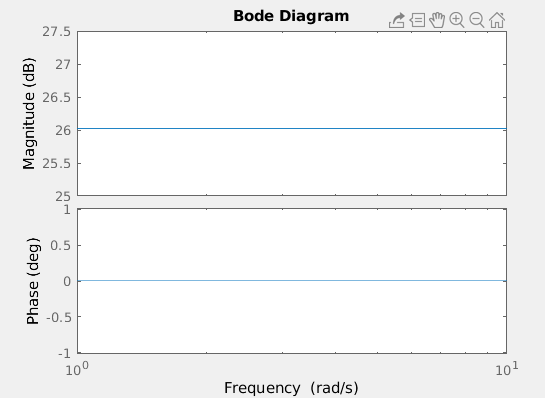
\includegraphics[scale=0.5]{./images/bode41.png}
		\end{figure}
		\newpage
		\item \textbf{Polo nell'origine: $\frac{1}{s^2}$}\\
		molteplicit\`a del polo: $\mu = 2$, quindi:\\
		$|\frac{1}{s^2}|_{dB} = -20\cdot\mu$ dB/dec = $-40$  dB/dec\\
		$\phi(\frac{1}{s^2}) = -\mu \cdot \phi(s) = -2 \cdot 90$\degree $= -180$\degree
		\begin{figure}[h!]
			\centering
			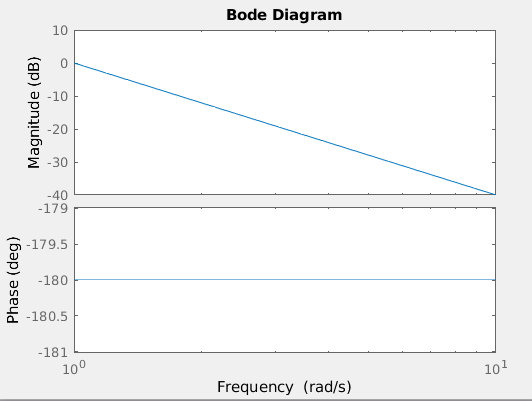
\includegraphics[scale=0.5]{./images/bode41_4.png}
		\end{figure}
		\item \textbf{Zeri complessi coniugati: $s^2 + 0.4s+1$}\vspace{5px}\\
		Lo studio degli zeri (poli) complessi coniugati richiede di conoscere pi\`u caratteristiche della funzione di trasferimento, ovvero: il valore della pulsazione naturale $\omega_n$, il coefficiente di smorzamento $\zeta$, il picco di risonanza $M_R$ e la pulsazione di risonanza $\omega_R$. Vediamo quindi come si calcolano.\\
		L'espressione degli zeri si presenta nella forma: $\frac{s^2}{\omega_n^2} + \frac{2\zeta}{\omega_n}s + 1$, da cui ricaviamo che:
		\begin{itemize}
			\item pulsazione naturale: $\omega_n^2 = 1$, quindi $\omega_n = 1 = 10^0$
			\item coefficiente di smorzamento: $\frac{2\zeta}{1} = 0.4$, quindi $\zeta = 0.2$
		\end{itemize} 
		Il diagramma della fase e quello del modulo restano costanti su 0 fino a $\omega_n$, dopodich\`e:\\
		$|s^2 + 0.4s+1|_{dB}$ = +40 dB/dec\\
		$\phi(s^2 + 0.4s+1)$ = +180\degree
		\begin{figure}[h!]
			\centering
			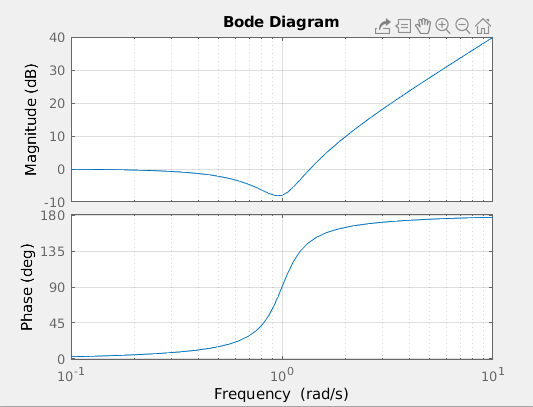
\includegraphics[scale=0.5]{./images/bode41_2.png}
		\end{figure}
		\vspace{5px}\\Dato che $0 \leq |\zeta| \leq \frac{\sqrt{2}}{2}$, e si tratta di zeri (quindi $\mu > 0$), il diagramma dei moduli ha un punto di \textit{minimo}, che viene chiamato \textit{picco di attenuazione}.\\Inoltre, dato che $\zeta < \frac{1}{2}$, il diagramma interseca l'ascissa \textit{a destra} di $\omega = \omega_n$.\\Il diagramma assume il suo valore minimo nel punto $\omega_R$:
		\[
			\omega_R = \omega_n\sqrt{1-2\zeta^2} = 0.95
		\]
		\\
		\item \textbf{Poli reali: $\frac{1}{1+10s}$}\vspace{5px}\\
		$\tau = \frac{1}{10} = 0.1$, quindi si ha un cambio di pendenza in $\omega_n = 0.1$:\vspace{5px}\\
		$|\frac{1}{1+10s}|_{dB} = -20log(1+10s) = -20 dB/dec$\\
		$\phi(\frac{1}{1+10s}) = -\phi(1+10s) = -90$\degree
		\begin{figure}[h!]
			\centering
			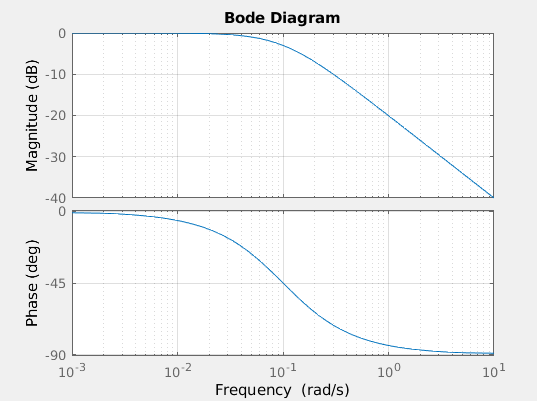
\includegraphics[scale=0.5]{./images/bode41_3.png}
		\end{figure}
	\end{itemize}
	\newpage
	\textbf{Diagramma totale}
	\begin{figure}[h!]
		\centering
		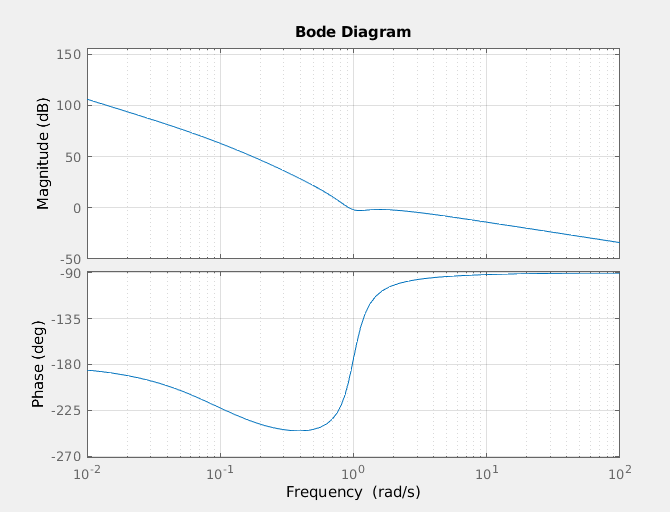
\includegraphics[scale=0.6]{./images/bode41tot.png}
	\end{figure}
	\newpage
	\paragraph*{Esercizio 4.2 - appello del 03/02/2017} Data la seguente funzione di trasferimento:
	\[
		G(s) = \frac{s^3(s+1)}{s^2+2s+3}
	\]
	Riportare la funzione in forma di Bode, disegnare i diagrammi delle singole componenti elementari e il diagramma globale.\\
	----------------------------------------------------------------------------------------------------------------------------\\Per portare la funzione in forma di Bode, \`e sufficiente "portare fuori" il 3 al denominatore, e otteniamo:
	\[
		G(s) = \frac{1}{3}s^3\frac{s+1}{\left(\frac{1}{3}s^2+\frac{2}{3}s+1\right)}
	\]
	Dobbiamo quindi tracciare i diagrammi di quattro componenti elementari: il termine costante $\frac{1}{3}$, lo zero nell'origine dato da $s^3$, lo zero reale in $s = -1$ e la coppia di poli complessi coniugati dati da $\left(\frac{1}{3}s^2+\frac{2}{3}s+1\right)$\\
	\begin{itemize}
		\item \textbf{Termine costante: $K_B = \frac{1}{3}$}\vspace{5px}\\
		$|K_B| = 20log_{10}(K_B) = -9.54$\\
		$\phi(K_B) = 0$\degree
		\begin{figure}[h!]
			\centering
			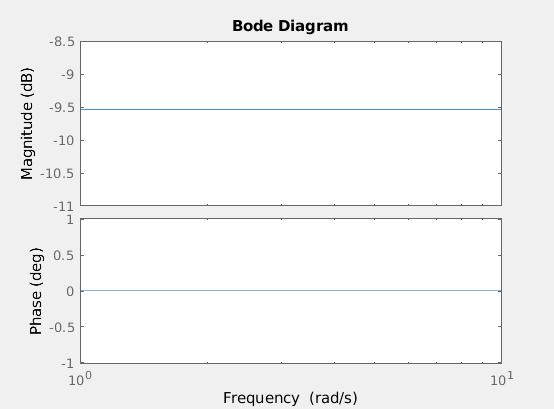
\includegraphics[scale=0.5]{./images/bode42_1.png}
		\end{figure}
		\newpage
		\item \textbf{Zero nell'origine: $s^3$}\vspace{5px}\\
		lo zero ha molteplicit\`a $\mu = 3$, di conseguenza:\\
		$|s^3|_{dB} = 20log(s^3) = 3 \cdot 20log(s) = 60log(s)$ = +60 dB/dec\\
		$\phi(s^3) = 3 \cdot \phi(s)= 3 \cdot 90$\degree $= +270$\degree
		\begin{figure}[h!]
			\centering
			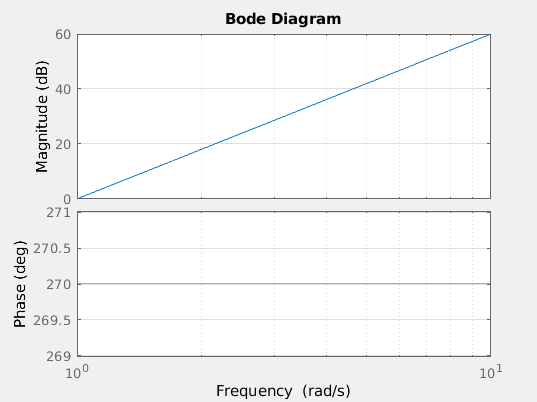
\includegraphics[scale=0.5]{./images/bode42_2.png}
		\end{figure}
		\item \textbf{Zeri reali: $(s+1)$}\\
		pulsazione naturale, $\omega_n$: dato che $\tau = 1$, ricaviamo che $\omega_n = \frac{1}{|\tau|} = 1$.\\Quindi il diagramma del modulo rimane costante fino su 0 fino a $\omega_n$, dopodic\`e il suo andamento sar\`a:\\
		$|s+1|_{dB} = 20log(s\tau) = 20log(s)$ = +20 dB/dec\\
		Per quanto riguarda il diagramma della fase, i cambi di pendenza si verificano alle pulsazioni:\\
		\[
		\omega_A = \frac{1}{4,81\tau}\quad\quad\quad\omega_B = \frac{4,81}{\tau}
		\]
		Nel nostro caso otteniamo $\omega_A \approx 0.20$ e $\omega_B = 4.81$.\\Questo significa che il diagramma della fase rimane costante su 0 fino alla pulsazione $\omega_A$, dopodich\`e cresce fino a raggiungere +90 in corrispondenza della pulsazione $\omega_B$.
		La fase aumenta di +90 perch\`e $(s+1)$ \`e uno zero di molteplicit\`a $\mu = 1$.
		\newpage
		\begin{figure}[h!]
			\centering
			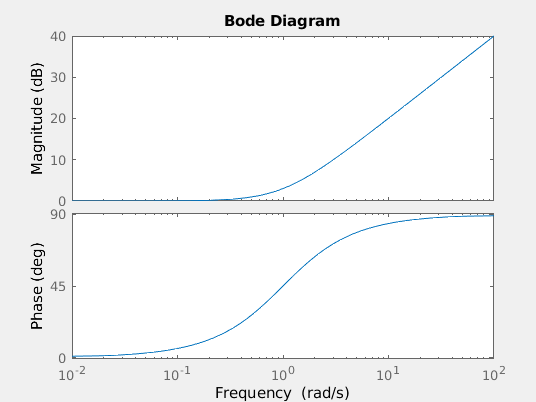
\includegraphics[scale=0.5]{./images/bode42_3.png}
		\end{figure}
		\item \textbf{Poli complessi coniugati: $\frac{1}{3}s^2 + \frac{2}{3}s + 1$}\vspace{5px}\\
		pulsazione naturale: $\omega_n^2 = 3$, quindi $\omega_n = \sqrt{3} = 1.73$\\
		coefficiente di smorzamento: $2\frac{\zeta}{\omega_n} = \frac{2}{3}\quad\rightarrow \quad\zeta = \frac{\sqrt{3}}{3} \approx 0.577$\\\\
		Dato che $0 \leq |\zeta| < \frac{\sqrt{2}}{2}$, deduciamo che il diagramma dei moduli ha un punto di \textit{massimo} (il picco di risonanza), e interseca l'ascissa \textit{a destra} della pulsazione naturale $\omega_n$.\\\\
		picco di risonanza: $M_R = \frac{1}{2\zeta\sqrt{1-\zeta^2}} \approx 1.06$\\
		pulsazione di risonanza: $\omega_R = \omega_n\sqrt{1-2\zeta^2} \approx 1.002$\vspace{5px}
		\begin{figure}[h!]
			\centering
			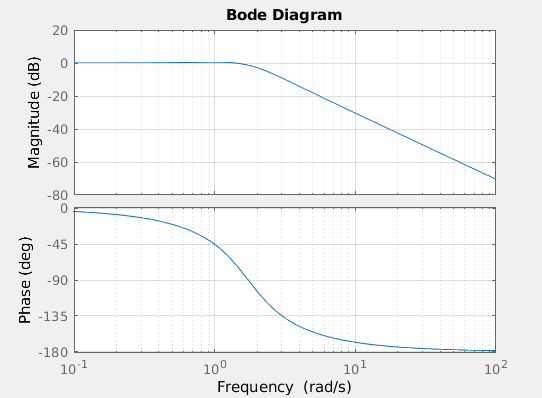
\includegraphics[scale=0.5]{./images/bode42_4.png}
		\end{figure}
		\newpage
		\textbf{Diagramma globale}\\
		\begin{figure}[h!]
			\centering
			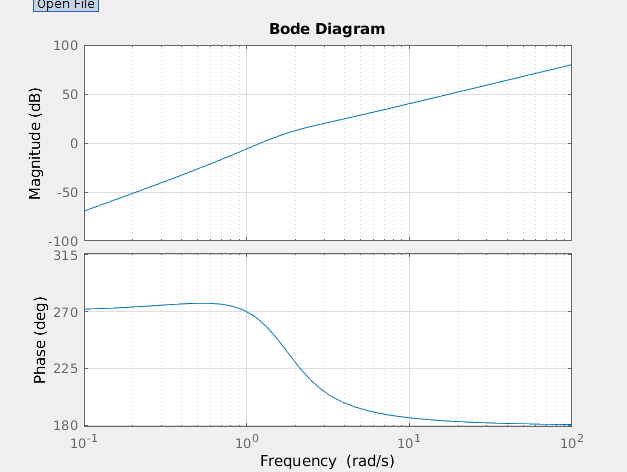
\includegraphics[scale=0.6]{./images/bode42_5.png}
		\end{figure}
	\end{itemize}
	\newpage
	\paragraph{Esercizio 4.3} Data la seguente funzione di trasferimento:
	\[
	G(s) = 100\frac{(s+1)}{(s+10)(s+100)}
	\]
	Riportare la funzione in forma di Bode, disegnare i diagrammi delle singole componenti elementari e il diagramma globale.\\
	---------------------------------------------------------------------------------------------------------------------\\ \\
	Forma di Bode: \quad$G(s) = \frac{100}{10 \cdot 100}\frac{s+1}{\left(0.1s+1\right)\left(0.01s+1\right)}$\quad$\rightarrow$\quad$G(s) = 0.1\frac{s+1}{\left(0.1s+1\right)\left(0.01s+1\right)}$\\\\
	Dalla forma di Bode si deduce che la funzione di trasferimento ha un termine costante, $K_B = 0.1$, uno zero in s = -1, un polo in s = -10 e un polo in s = -100.\\Procediamo quindi tracciando i diagrammi delle componenti elementari.\\
	\begin{itemize}
		\item \textbf{Termine costante, $K_B = 0.1$}\vspace{5px}\\
		$|K_B|_{dB} = 20log(0.1) = -20$ dB/dec\\
		$\phi(K_B) = 0$\degree
		\begin{figure}[h!]
			\centering
			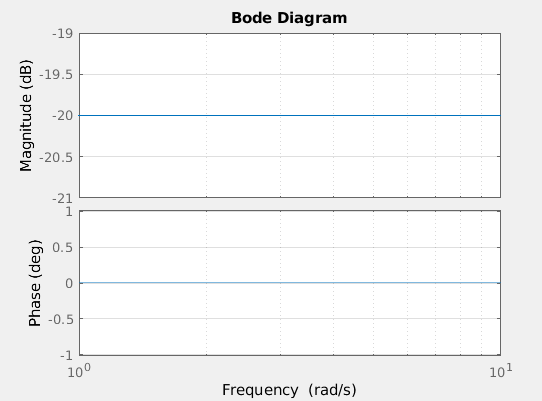
\includegraphics[scale=0.5]{./images/bode43_1.png}
		\end{figure}
		\newpage
		\item \textbf{Zero reale, $(s+1)$}\vspace{5px}\\
		$\tau = 1$, quindi il diagramma del modulo rimane costante su 0 fino alla pulsazione $\omega_n = \frac{1}{|\tau|} = 1$. Dopodich\`e, la pendenza diventa:\vspace{5px}\\
		$|s+1|_{dB} = 20log(s\tau) = 20log(s)$ = 20 db/dec\vspace{5px}\\
		Nel diagramma delle fasi, i cambi di pendenza avvengono alle pulsazioni $\omega_A = \frac{1}{4.81\tau} \approx 0.20$ e $\omega_B = \frac{4.81}{\tau} = 4.81$, dopodich\`e il diagramma si stabilizza alla fase:\vspace{5px}\\
		$\phi(s+1) = +90$\degree
		\begin{figure}[h!]
			\centering
			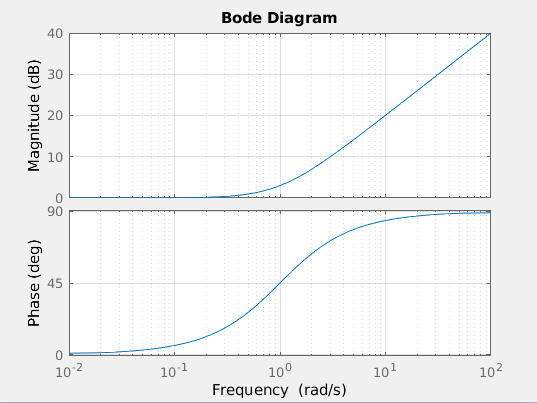
\includegraphics[scale=0.5]{./images/bode43_2.png}
		\end{figure}
		\item \textbf{Polo reale, $\frac{1}{0.1s+1}$}\vspace{5px}\\
		$\tau = 0.1$, quindi il diagramma del modulo rimane costante su 0 fino alla pulsazione $\omega_n = \frac{1}{|\tau|} = 10$. Dopodich\`e la pendenza diventa:\vspace{5px}\\
		$|\frac{1}{0.1s+1}|_{dB} = 20log\left(\frac{1}{0.1s+1}\right) = -20log(0.1s+1) \approx -20log(0.1s) \approx$ -20 dB/dec\vspace{5px}\\
		Nel diagramma delle fasi, i cambi di pendenza avvengono alle pulsazioni $\omega_A = \frac{1}{4.81\tau} \approx 2.07$ e $\omega_B = \frac{4.81}{\tau} = 48.1$, dopodich\`e il diagramma si stabilizza alla fase:\vspace{5px}\\
		$\phi\left(\frac{1}{0.1s+1}\right) = -\phi(0.1s+1) = -90$\degree
		\newpage
		\begin{figure}[h!]
			\centering
			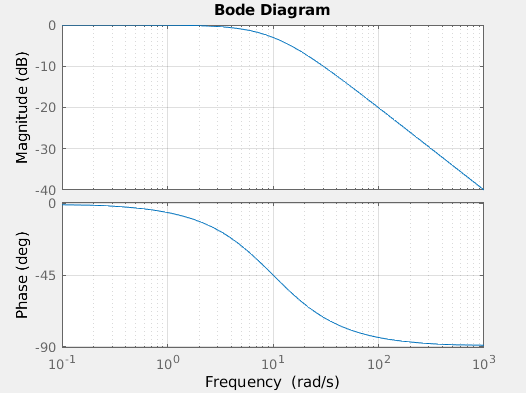
\includegraphics[scale=0.5]{./images/bode43_4.png}
		\end{figure}
		\item \textbf{Polo reale, $\frac{1}{0.01s+1}$}\vspace{5px}\\
		$\tau = 0.01$, quindi la pulsazione naturale vale $\omega_n = 100$. Il diagramma dei moduli rimane quindi costante su 0 fino alla pulsazione $\omega_n$, dopodich\`e diminuisce:\vspace{5px}\\
		$|\frac{1}{0.01s+1}|_{dB} = 20log\left(\frac{1}{0.01s+1}\right) = -20log(0.01s+1) \approx -20log(0.01s)\approx$ -20 dB/dec\vspace{5px}\\Per quanto riguarda la fase, il diagramma resta costante su 0 fino alla pulsazione $\omega_A = \frac{1}{4.81\tau}$, dopodich\`e aumenta fino a raggiungere la fase +90 in corrispondenza della pulsazione $\omega_B = \frac{4.81}{\tau}$
		\begin{figure}[h!]
			\centering
			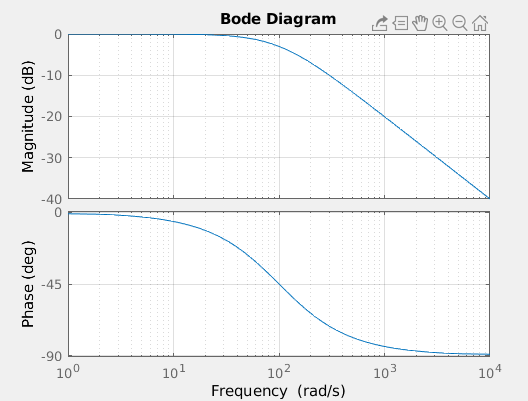
\includegraphics[scale=0.5]{./images/bode43_5.png}
		\end{figure}
	\end{itemize}
	\newpage
	Ora abbiamo tutti gli elementi per tracciare il diagramma globale della nostra funzione di trasferimento:\\ \\
	\textbf{Diagramma globale}
	\begin{figure}[h!]
		\centering
		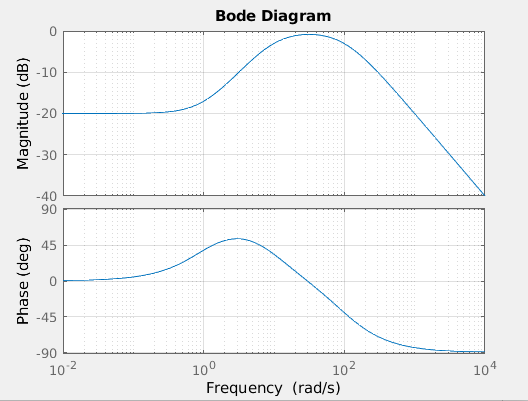
\includegraphics[scale=0.6]{./images/bode43tot.png}
	\end{figure}
	\newpage
	\paragraph*{Esercizio 4.4} Data la seguente funzione di trasferimento:
	\[
		H(s) = 30\frac{(s+10)}{s^2+3s+50}
	\]
	Riportare la funzione in forma di Bode, disegnare i diagrammi delle singole componenti elementari e il diagramma globale.\\
	---------------------------------------------------------------------------------------------------------------------\\ \\
	Forma di Bode:
	\[
		H(s) = 30\frac{10}{50}\frac{\left(\frac{1}{10}s+1\right)}{\left(\frac{1}{50}s^2+\frac{3}{50}s+1\right)} = 6\frac{\left(\frac{1}{10}s+1\right)}{\left(\frac{1}{50}s^2+\frac{3}{50}s+1\right)} 
	\]
	Quindi abbiamo tre componenti elementari di cui tracciare il diagramma: il termine costante, $K_B = 6$, uno zero in $s = -10$ e due poli complessi coniugati dati da $\left(\frac{1}{50}s^2+\frac{3}{50}s+1\right)$\\
	\begin{itemize}
		\item \textbf{Termine costante, $K_B$}\vspace{5px}\\
		$|K_B|_{dB} = 20log(K_B) = 15.56$\\
		$\phi(K_B) = 0$\degree
		\begin{figure}[h!]
			\centering
			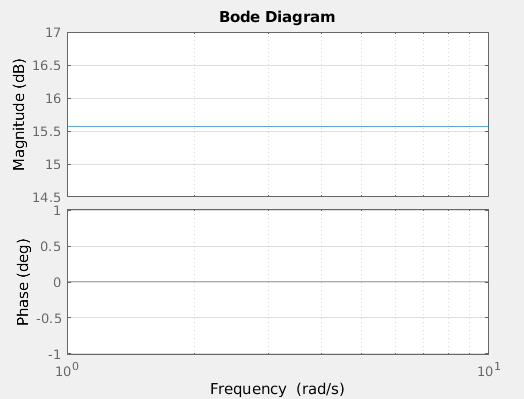
\includegraphics[scale=0.5]{./images/bode44_1.png}
		\end{figure}
	\newpage
		\item \textbf{Zeri reali, $(\frac{1}{10}s + 1)$}\vspace{5px}\\
		$\tau = \frac{1}{10}$, quindi il diagramma del modulo resta costante su 0 fino alla pulsazione $\frac{1}{|\tau|} = 10$, dopodich\`e varia nel seguente modo:\vspace{5px}\\
		$|\frac{1}{10}s + 1|_{dB} = 20log(\frac{1}{10}s + 1) =$ +20 dB/dec\vspace{5px}\\
		Il diagramma della fase, invece, subisce i cambi di pendenza in corrispondenza delle pulsazioni:
		\[
			\omega_A = \frac{1}{4.81\tau} = 2.07\quad\quad\quad\omega_B = \frac{4.81}{\tau} = 48.1
		\]
		Prima della pulsazione $\omega_A$ il diagramma resta costante su 0. Dopodich\`e, cresce fino a raggiungere la fase +90 in corrispondenza della pulsazione $\omega_B$.\\Perch\`e cresce a +90? Perch\`e \`e uno \textit{zero}, e come tale porta a un \textit{aumento} di fase, e la sua molteplicit\`a \`e $\mu = 1$, quindi l'aumento di fase vale $+90 \cdot \mu$.
		\begin{figure}[h!]
			\centering
			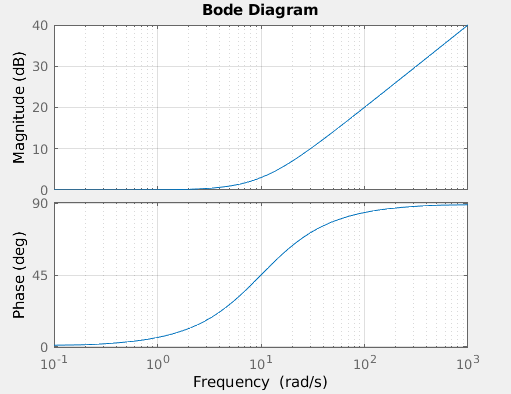
\includegraphics[scale=0.5]{./images/bode44_2.png}
		\end{figure}
		\item \textbf{Poli complessi coniugati}, $\left(\frac{1}{50}s^2+\frac{3}{50}s+1\right)$\vspace{5px}\\
		Per disegnare accuratamente il diagramma dei moduli abbiamo bisogno di calcolare: la pulsazione naturale $\omega_n$, il coefficiente di smorzamento $\zeta$, il picco di risonanza $M_R$ e la pulsazione di risonanza.\\I primi due elementi si ricavano facilmente sapendo che, quando la funzione di trasferimento \`e in forma di Bode, i poli complessi coniugati sono nella forma: $\frac{s^2}{\omega_n^2} + \frac{2\zeta}{\omega_n}s + 1$. Quindi:
		\begin{itemize}
			\item pulsazione naturale: $\omega_n^2 = 50 \rightarrow \omega_n = \sqrt{50} \approx 7.07$ 
			\item coefficiente di smorzamento: $\frac{2\zeta}{\omega_n} = \frac{3}{50} \rightarrow \frac{2\zeta}{\sqrt{50}} = \frac{3}{50} \rightarrow \zeta = \frac{3}{50} \cdot \frac{\sqrt{50}}{2} = \frac{3}{2\sqrt{50}} \approx0.212$
		\end{itemize}
		Dato che $0 \leq |\zeta| \leq \frac{\sqrt{2}}{2}$, e la molteplicit\`a \`e $\mu = -1 < 0$, deduciamo che il diagramma delle fasi avr\`a un punto di \textit{massimo} (individuato dal picco di risonanza) e intersecher\`a l'ascissa \textit{a destra} di $\omega_n$.\\
		Calcoliamo ora il picco di risonanza $M_R$ e la pulsazione di risonanza $\omega_R$:
		\[
			M_R = \frac{1}{2\zeta\sqrt{1-\zeta^2}} \approx 0.414\quad\quad\quad\omega_R = \omega_n\sqrt{1-2\zeta^2} \approx 6.74
		\]
		Per studiare la fase, invece, \`e sufficiente calcolare le pulsazioni alle quali si verifica il cambio di fase:
		\[
			\omega_A = \frac{\omega_n}{4.81^\zeta} \approx 5.06\quad\quad\quad\omega_B = \omega_n \cdot 4.81^\zeta \approx 9.86
		\]
		Quindi il diagramma della fase resta costante su 0 fino a $\omega_A$, dopodich\`e cresce fino a raggiungere -180\degree in corrispondenza della pulsazione $\omega_B$.
		Ora abbiamo tutti gli elementi necessari per disegnare i diagrammi:\vspace{10px}
		\begin{figure}[h!]
			\centering
			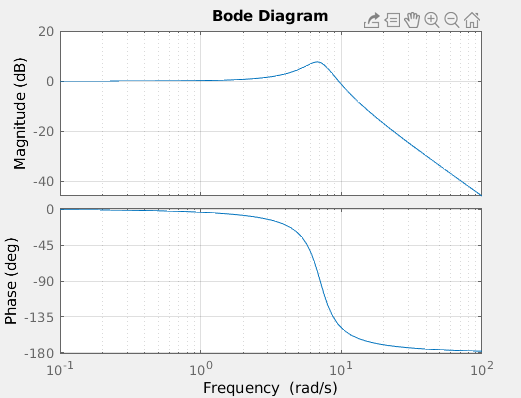
\includegraphics[scale=0.5]{./images/bode44_3.png}
		\end{figure}
		\\Ora abbiamo tutti gli elementi per poter disegnare il diagramma totale della nostra funzione di trasferimento (vedi pagina seguente).
		\newpage
		\textbf{Diagramma totale}
		\begin{figure}[h!]
			\centering
			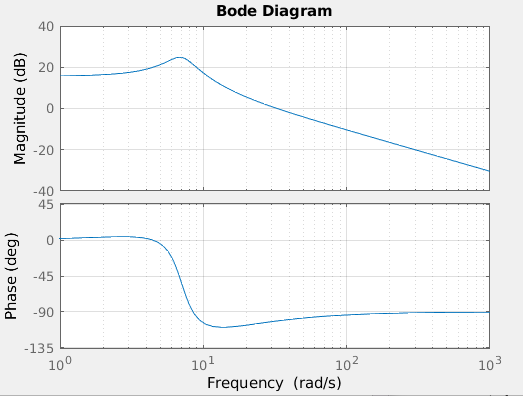
\includegraphics[scale=0.6]{./images/bode44tot.png}
		\end{figure}
	\end{itemize}
	\newpage
	\paragraph{Esercizio 4.5} Data la seguente funzione di trasferimento:
	\[
		H(s) = \frac{(s+1)(s^2+2s+9)}{s^3}
	\]
	Riportare la funzione in forma di Bode, disegnare i diagrammi delle singole componenti elementari e il diagramma globale.\\
	---------------------------------------------------------------------------------------------------------------------\\ \\
	Forma di Bode:
	\[
		H(s) = \frac{9(s+1)\left(1+\frac{2}{9}s+\frac{1}{9}s^2\right)}{s^3}\quad\rightarrow\quad H(s) = 9 \cdot \frac{1}{s^3}\cdot (1+s)\left(1+\frac{2}{9}s+\frac{1}{9}s^2\right)
	\]
	Quindi abbiamo quattro componenti elementari di cui dobbiamo disegnare i diagrammi: il termine costante $K_B = 9$, il polo nell'origine $\frac{1}{s^3}$, lo zero reale $(1+s)$ e infine gli zeri complessi coniugati $\left(1+\frac{2}{9}s+\frac{1}{9}s^2\right)$.\\
	\begin{itemize}
		\item \textbf{Termine costate}, $K_B = 9$\vspace{5px}\\
		$|K_B|_{dB} = 20log(9) = 19.08$\\
		$\phi(K_B) = 0$\degree
		\begin{figure}[h!]
			\centering
			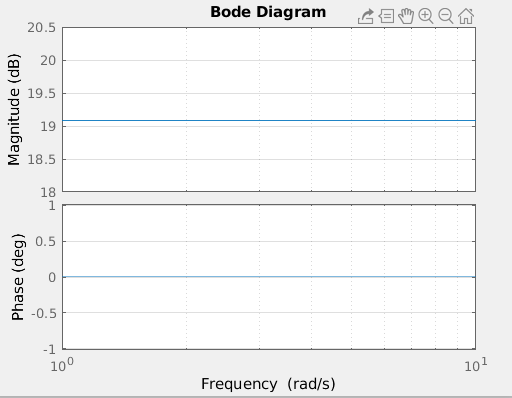
\includegraphics[scale=0.5]{./images/bode45_1.png}
		\end{figure}
		\item \textbf{Polo nell'origine}, $\frac{1}{s^3}$\vspace{5px}\\
		$\left|\frac{1}{s^3}\right|_{dB} = 20log\left(\frac{1}{s^3}\right) = -3 \cdot 20log(s) = -60$ dB/dec\vspace{5px}\\
		$\phi\left(\frac{1}{s^3}\right) = -3 \cdot \phi(s) = -3 \cdot 90$\degree = -270\degree
		\begin{figure}[h!]
			\centering
			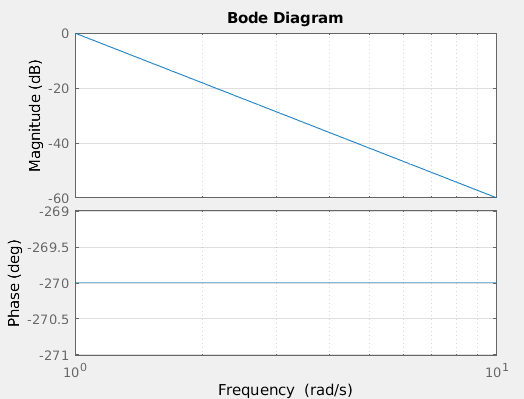
\includegraphics[scale=0.5]{./images/bode45_2.png}
		\end{figure}
		\item \textbf{Zero nell'origine}, $(1+s)$\vspace{5px}\\
		$\tau = 1$, quindi il diagramma dei moduli resta costante su 0 fino a $\omega = \frac{1}{|\tau|} = 1$ (detto anche \textit{punto di rottura}), dopodich\`e varia in pendenza:\\
		$|1+s|_{dB} = 20log(1+s) = +20$ dB/dec\\
		Per quanto riguarda la fase, i cambiamenti di pendenza avvengono alle pulsazioni:
		\[
			\omega_A = \frac{1}{4.81\tau}\approx0.20\quad\quad\quad\omega_B = \frac{4.81}{\tau} = 4.81
		\]
		Il diagramma resta costante fino a $\omega_A$, dopodich\`e la pendenza aumenta fino a raggiungere +90\degree in corrispondenza di $\omega_B$.
		\begin{figure}[h!]
			\centering
			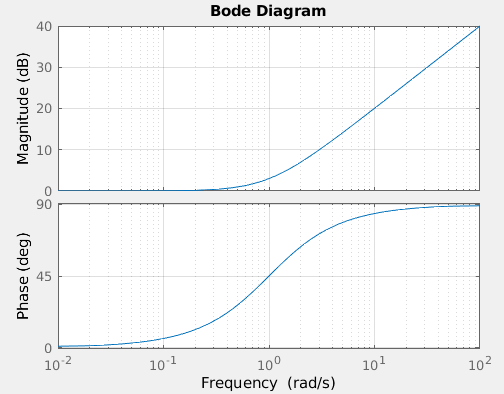
\includegraphics[scale=0.5]{./images/bode45_3.png}
		\end{figure}
		\item \textbf{Zeri complessi coniugati}, $\left(1+\frac{2}{9}s + \frac{1}{9}s^2\right)$\vspace{5px}\\
		Calcoliamo per prima cosa il valore della pulsazione naturale $\omega_n$ e il coefficiente di smorzamento $\zeta$:
		\begin{itemize}
			\item pulsazione naturale: $\omega_n^2 = 9 \rightarrow \omega_n = \sqrt{9} = 3$
			\item coefficiente di smorzamento: $\frac{2\zeta}{\omega_n} = \frac{2}{9} \rightarrow \zeta = \frac{1}{3} \approx 0.33$
		\end{itemize}
		Dato che $0 \leq |\zeta| \leq \frac{\sqrt{2}}{2}$ e la molteplicit\`a $\mu$ di questo termine \`e positiva, concludiamo che il diagramma ha un punto di \textit{minimo}. Inoltre, dato che $0 \leq |\zeta| \leq \frac{1}{2}$, il diagramma interseca l'ascissa \textit{a destra} della pulsazione $\omega_n = 3$.\\
		Il diagramma assume il suo valore minimo in corrispondenza della pulsazione di attenuazione $\omega_R$:
		\[
			\omega_R = \omega_n\sqrt{1-2\zeta^2} \approx 1.73
		\]
		Quindi all'inizio il modulo \`e a quota 0, dopodich\`e comincia a calare fino a raggiungere il suo valore minimo in corrispondenza del punto $\omega_R = 1.73$. Passato questo punto, riprende a salire fino a stabilizzarsi sulla retta +40 dB/dec.\\
		Per quanto riguarda la fase, invece, i cambi di pendenza avvengono in corrispondenza delle pulsazioni:
		\[
			\omega_A = \frac{\omega_n}{4.81^\zeta} \approx 1.78\quad\quad\quad\omega_B = \omega_n \cdot 4.81^\zeta \approx 5.03
		\]
		Quindi la fase resta costante su 0\degree fino a $\omega_A$, dopodich\`e cresce fino a raggiungere la fase +180\degree in corrispondenza della pulsazione $\omega_B$.\\
		\begin{figure}[h!]
			\centering
			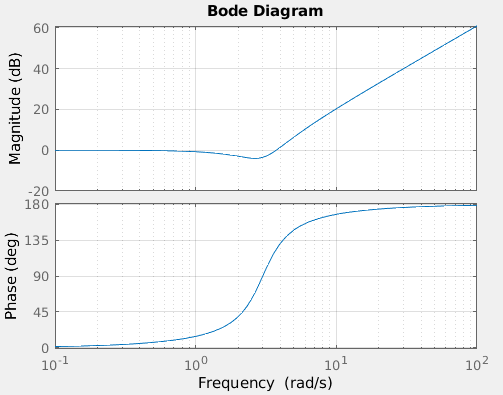
\includegraphics[scale=0.5]{./images/bode45_4.png}
		\end{figure}
	\end{itemize}
	\newpage
	\textbf{Diagramma totale}
	\begin{figure}[h!]
		\centering
		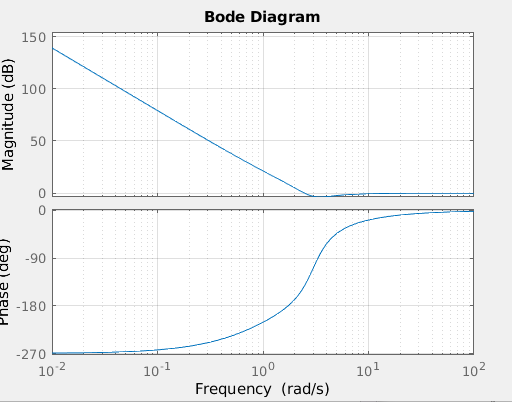
\includegraphics[scale=0.6]{./images/bode45tot.png}
	\end{figure}
	\newpage
	\paragraph{Esercizio 4.6 - appello del 01/07/2019} Data la seguente funzione di trasferimento:
	\[
		G(s) = \frac{10(s^2+4)}{s(s+3)(s^2+3s+4)}
	\]
	disegnare il diagramma di Bode (sia di ciascuna componente elementare, sia il risultante diagramma globale).\\
	---------------------------------------------------------------------------------------------------------------------\\ \\
	Scriviamo la funzione di trasferimento in forma di Bode:
	\[
		G(s) = \frac{10 \cdot 4}{3 \cdot 4}\cdot\frac{1+\frac{1}{4}s^2}{s\left(1+\frac{1}{3}s\right)\left(1+\frac{3}{4}s+\frac{1}{4}s^2\right)}\quad\rightarrow\quad G(s) = \frac{10}{3}\cdot\frac{1}{s}\cdot\frac{1+\frac{1}{4}s^2}{\left(1+\frac{1}{3}s\right)\left(1+\frac{3}{4}s+\frac{1}{4}s^2\right)}
	\]
	Quindi abbiamo cinque componenti elementari di cui tracciare il grafico.\\
	\begin{itemize}
		\item \textbf{Termine costante}, $K_B = \frac{10}{3}$\vspace{5px}\\
		$|K_B|_{dB} = 20log\left(\frac{10}{3}\right) = 10.45$\\
		$\phi(K_B) = 0$\degree
		\begin{figure}[h!]
			\centering
			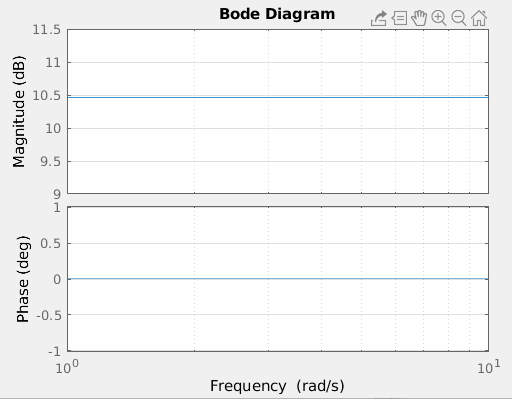
\includegraphics[scale=0.5]{./images/bode46_1.png}
		\end{figure}
		\item \textbf{Polo nell'origine}, $\frac{1}{s}$\vspace{5px}\\$\left|\frac{1}{s}\right|_{dB} = -20$ dB/dec\\
		$\phi\left(\frac{1}{s}\right) = -90$\degree
		\begin{figure}[h!]
			\centering
			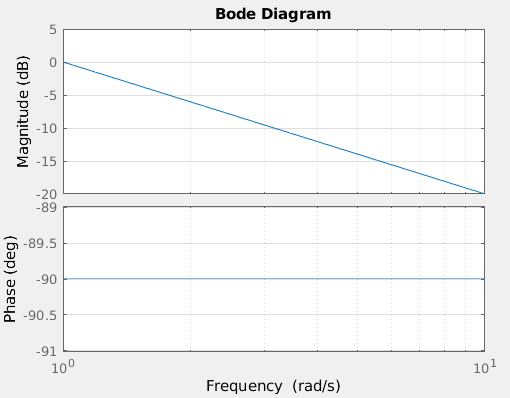
\includegraphics[scale=0.5]{./images/bode46_2.png}
		\end{figure}
		\newpage
		\item \textbf{Zeri complessi coniugati}, $1+\frac{1}{4}s^2$\vspace{5px}\\
		Calcoliamo la pulsazione naturale, che rappresenta il punto di rottura del diagramma (ovvero il punto in cui si ha una variazione di pendenza):
		\[
			\omega_n^2 = 4 \rightarrow \omega_n = 2
		\]
		Quindi sia il diagramma del modulo che quello della fase restano costanti su 0 fino a $\omega_n$, dopodich\`e si ha che:\\
		$\left|1+\frac{1}{4}s^2\right|_{dB} = +40$ dB/dec\\
		$\phi\left(1+\frac{1}{4}s^2\right) = +180$\degree
		\begin{figure}[h!]
			\centering
			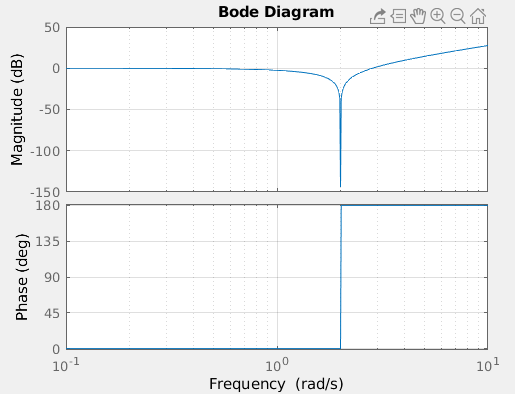
\includegraphics[scale=0.5]{./images/bode46_3.png}
		\end{figure}
		\\Notare l'andamento "a gradino" del diagramma della fase: questo \`e dovuto al fatto che il coefficiente di smorzamento $\zeta$ \`e pari a 0! Infatti, nell'espressione degli zeri complessi coniugati manca il termine $\frac{2\zeta}{\omega_n}s$. Pi\`u il valore di $\zeta$ si avvicina a 0, pi\`u il cambiamento di fase sar\`a "brusco". Al contrario, se $\zeta$ si avvicina a 1, il cambiamento di fase seguir\`a asintoticamente l'andamento del gradino, ma sar\`a pi\`u "dolce".
		\item \textbf{Poli reali}, $1 + \frac{1}{3}s$\vspace{5px}\\
		Dato che $\tau = \frac{1}{3}$, il valore della pulsazione naturale sar\`a: $\omega_n = \frac{1}{|\tau|} = 3$.\\
		A partire da $\omega_n$ si ha quindi che:\\
		$\left|1 + \frac{1}{3}s\right|_{dB} = -20$ dB/dec\\
		$\phi\left(1 + \frac{1}{3}s\right) = -90$\degree
		\begin{figure}[h!]
			\centering
			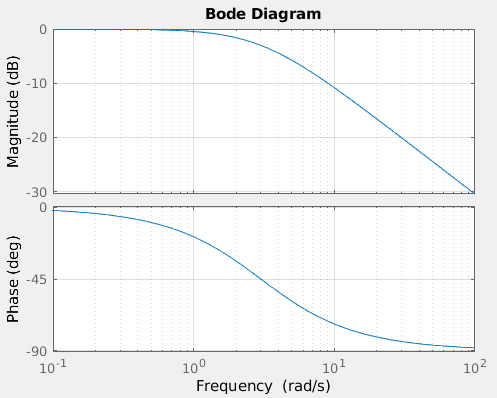
\includegraphics[scale=0.5]{./images/bode46_4.png}
		\end{figure}
		\item \textbf{Poli complessi coniugati}, $1+\frac{3}{4}s + \frac{1}{4}s^2$
		\begin{itemize}
			\item pulsazione naturale: $\omega_n^2 = 4 \rightarrow \omega_n = 2$
			\item coefficiente di smorzamento: $\frac{2\zeta}{\omega_n} = \frac{3}{4} \rightarrow \zeta = \frac{3}{4} = 0.75$
		\end{itemize}
		Il valore del coefficiente di smorzamento \`e abbastanza vicino a 1, quindi ci aspettiamo un cambiamento di fase meno brusco rispetto a quello degli zeri complessi coniugati visti prima.\\
		Notiamo che $\frac{\sqrt{2}}{2} \leq |\zeta| \leq 1$, quindi il diagramma \textit{non interseca mai l'ascissa}. Inoltre, visto che si tratta di poli, e quindi $\mu < 0$, concludiamo che il diagramma si trova interamente \textit{al di sotto} della sua approssimazione asintotica (viceversa, se si fosse trattato di zeri, il diagramma si sarebbe trovato interamente \textit{al di sopra} dell'approssimazione).
		\newpage
		\begin{figure}[h!]
			\centering
			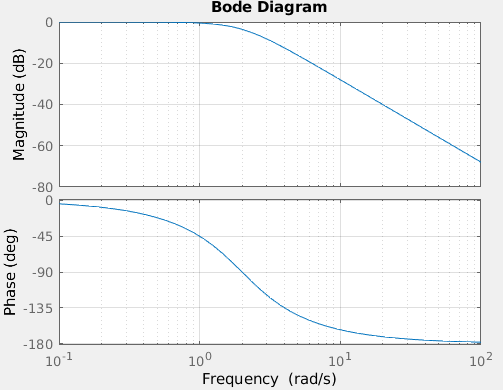
\includegraphics[scale=0.5]{./images/bode46_5.png}
		\end{figure}
	\end{itemize}
	Ora possiamo disegnare il diagramma globale della funzione di trasferimento:\\\\
	\textbf{Diagramma globale}
	\begin{figure}[h!]
		\centering
		\includegraphics[scale=0.6]{./images/bode46tot.png}
	\end{figure}
	\newpage
	\section*{Trasformate di Fourier}
	\paragraph{Esercizio 5.1 - parziale del 13/06/2019} Dato il seguente schema a blocchi trovare l’uscita v(t) del sistema per via grafica lavorando nel dominio delle frequenze:
	\begin{figure}[h!]
		\centering
		\includegraphics[scale=0.4]{./images/fourier51.png}
	\end{figure}
	\\Dove $u(t) = 3cos(6\pi t) + cos(2\pi t)$, $w(t) = 2cos(4\pi t)$, $h(t) = 4sinc(4t)$, $f(t) = 2sinc(2t)$.\\
	Periodo di campionamento con $T= 1s$. \\Si verifica il fenomeno di aliasing?  Motivare la risposta.\\ \\
	----------------------------------------------------------------------------------------------------------------------------\\
	Dobbiamo convertire i segnali dati dal dominio del tempo al dominio delle frequenze, quindi calcoliamo di ognuno la trasformata di Fourier:\\\\
	$u(t) = 3cos(6\pi t) + cos(2\pi t)\quad\xRightarrow[]{TdF}\quad U(f) = \frac{3}{2}\left[\delta(f-3) + \delta(f+3)\right] + \frac{1}{2}\left[\delta(f-1) + \delta(f+1)\right]$\\\\
	$w(t) = 2cos(4\pi t)\quad\xRightarrow[]{TdF}\quad W(f) = \delta(f-2) + \delta(f+2)$\\\\
	$h(t) = 4sinc(4t)\quad\xRightarrow[]{TdF}\quad H(f) = \Pi\left(\frac{f}{4}\right)$\\\\
	$f(t) = 2sinc(2t)\quad\xRightarrow[]{TdF}\quad F(f) = \Pi\left(\frac{f}{2}\right)$\\\\
	frequenza di campionamento: $f_c = 1$ Hz\\\\
	Ora disegniamo i due segnali di input, ovvero $U(f)$ e $W(f)$:
	\begin{figure}[h!]
		\centering
		\includegraphics[scale=0.6]{./images/fourier52.png}
	\end{figure}
	\\Dopodich\`e effettuiamo la convoluzione dei due segnali, ottenendo il segnale risultante $V_1(f)$. La convoluzione tra due segnali per via grafica si realizza andando a "centrare" un segnale nell'altro. In questo caso, scegliamo arbitrariamente di centrare il segnale $U(f)$ in $W(f)$, ma si potrebbe anche fare il contrario.\\Se i segnali si sovrappongono, bisogna \textbf{sommare} le ampiezze, altrimenti bisogna \textbf{moltiplicarle}.
	\begin{figure}[h!]
		\centering
		\includegraphics[scale=0.4]{./images/fourier53.png}
	\end{figure}
	\\Ora dobbiamo applicare il filtro $H(f)$, che \`e una box di ampiezza $A=1$ e banda $B=2$: teniamo solo la parte di $V_1(f)$ che viene inclusa dalla box.
	\begin{figure}[h!]
		\centering
		\includegraphics[scale=0.4]{./images/fourier54.png}
	\end{figure}
	\\L'ampiezza del segnale risultante $V_2(f)$ si ricava \textbf{moltiplicando} l'ampiezza del filtro e quella del segnale. In questo caso, $A_H = 1$, $A_{V_1} = 2$, quindi l'ampiezza del segnale risultante $V_2(f)$ sar\`a 2:
	\begin{figure}[h!]
		\centering
		\includegraphics[scale=0.4]{./images/fourier55.png}
	\end{figure}
	\\Adesso dobbiamo campionare il segnale a 1 Hz. \\Ricordiamo che \textit{un campionamento nel tempo corrisponde a una replicazione nelle frequenze}! Visto che stiamo lavorando nel dominio delle frequenze, andremo a replicare il segnale $V_2(f)$ a frequenza 1 Hz, ottenendo il segnale $V_3(f)$.\\Se durante la replicazione i segnali si sovrappongono, significa che abbiamo \textbf{aliasing} e dobbiamo sommare le ampiezze dei due segnali (parlando in termini prettamente grafici, andiamo a posizionare un segnale sopra l'altro):
	\begin{figure}[h!]
		\centering
		\includegraphics[scale=0.4]{./images/fourier56.png}
	\end{figure}
	\\In questo caso notiamo subito che \textbf{si verifica il fenomeno di aliasing}.\\ Avere aliasing significa che, dopo aver effettuato il campionamento, i segnali diventano indistinguibili (perché si sovrappongono!) e dunque non è possibile avere un filtro di ricostruzione che restituisca i segnali originali.\\La condizione da rispettare per evitare aliasing viene enunciata nel \textit{teorema del campionamento} ed è che la frequenza di campionamento sia superiore al doppio della banda del segnale:
	\[
		f_c > 2\cdot B
	\]
	dove B rappresenta la banda del segnale. In questo caso, $B = 1$ e $f_c = 1Hz$, quindi evidentemente la condizione non è rispettata.\\\\L'ultimo passaggio che dobbiamo fare \`e filtrare questo segnale con $F(f)$, tenendo solo la parte di segnale che risulta inclusa nel filtro, e moltiplicando le ampiezze.\\
	\begin{figure}[h!]
		\centering
		\includegraphics[scale=0.4]{./images/fourier57.png}
	\end{figure}
	\\Il filtro $F(f)$ ha ampiezza $A_F=2$ e banda $B_F=1$, quindi l'ampiezza del segnale risultante $V(f)$ sar\`a $A_f = 8$.\\Si noti che il segnale risultante comprende anche la parte di $V_3(f)$ presente ai "bordi" del filtro.
	\begin{figure}[h!]
		\centering
		\includegraphics[scale=0.4]{./images/fourier58.png}
	\end{figure}
	\\L'equazione del segnale risultante nel dominio delle frequenze è:
	\[
		V(f) = 4\delta(f) + 4[\delta(f-1) + \delta(f+1)]
	\]
	Eseguendo l'antitrasformata otteniamo il segnale nel dominio del tempo:
	\[
		v(t) =  4 + 8cos(2\pi t)
	\]
	\newpage
	\paragraph{Esercizio 5.2 - appello 01/07/2019}
	Dato il seguente schema a blocchi trovare l’uscita $v(t)$ del sistema per via grafica lavorando nel dominio delle frequenze:
	\begin{figure}[h!]
		\centering
		\includegraphics[scale=0.4]{./images/fourier21.png}
	\end{figure}
	\\Dove $u(t) = sinc(2t) + 2$, $w(t) = 4cos(10\pi t)$, $h(t) = 4sinc(10t)$, $f(t) = 2sinc(2t)$. \\Periodo di campionamento con $T=110s$.\\Si verifica il fenomeno di Aliasing? Motivare la risposta.
	\\\\
----------------------------------------------------------------------------------------------------------------------------\\
	Per prima cosa, scriviamo le trasformate di Fourier dei segnali:\\
	$u(t) = sinc(2t) + 2\quad\xRightarrow[]{TdF}\quad U(f) = \frac{1}{2}\Pi\left(\frac{f}{2}\right) + 2\delta(f)$\\
	$w(t) = 4cos(10\pi t)\quad\xRightarrow[]{TdF}\quad W(f) = 2\left[\delta(f-5) + \delta(f+5)\right]$\\
	$h(t) = 4sinc(10t)\quad\xRightarrow[]{TdF}\quad H(f) = \frac{4}{10}\Pi\left(\frac{f}{10}\right)$\\
	$f(t) = 2sinc(2t)\quad\xRightarrow[]{TdF}\quad F(f) = \Pi\left(\frac{f}{2}\right)$\vspace{5px}\\
	periodo di campionamento: $T=110s\quad\rightarrow\quad$ frequenza di campionamento: $f_c = \frac{1}{T} = 10Hz$.\\\\
	Ora disegnamo i grafici dei segnali in ingresso, $U(f)$ e $W(f)$:
	\begin{figure}[h!]
		\centering
		\includegraphics[scale=0.4]{./images/fourier22.png}
	\end{figure}
	\\Eseguiamo per via grafica la convoluzione tra i due, andando a centrare il segnale $U(f)$ in $W(f)$ e ottenendo così il segnale risultante $V_1(f)$.\\L'ampiezza di $V_1(f)$ si ottiene moltiplicando le ampiezze di $U(f)$ e $W(f)$.
	\newpage
	\begin{figure}[h!]
		\centering
		\includegraphics[scale=0.4]{./images/fourier23.png}
	\end{figure}
	Il segnale $V_2(f)$ si ottiene applicando il filtro $H(f)$ (banda $B_H = 5$ e ampiezza $A_H = \frac{2}{5}$) su $V_1(f)$: teniamo solo la parte di segnale che viene inclusa dal filtro (\textit{estremi inclusi!}) e moltiplichiamo le loro ampiezze.
	\begin{figure}[h!]
		\centering
		\includegraphics[scale=0.4]{./images/fourier24.png}
	\end{figure}
	\\Da cui otteniamo:
	\begin{figure}[h!]
		\centering
		\includegraphics[scale=0.4]{./images/fourier25.png}
	\end{figure}
	\\Ora dobbiamo eseguire il campionamento a $T = 110s$: lavorando nelle frequenze, questo significa replicare il segnale ogni $f_c = 10Hz$.\\Notiamo subito che la banda del segnale $V_2(f)$ è $B_{V_2} = 5$, e quindi la condizione $f_c > 2\cdot B$ non è rispettata: significa che \textbf{si verifica il fenomeno di aliasing} (teorema del campionamento).\\Questa conclusione viene confermata dal grafico del segnale risultante, in cui notiamo un'evidente sovrapposizione di segnali:
	\begin{figure}[h!]
		\centering
		\includegraphics[scale=0.4]{./images/fourier26.png}
	\end{figure}
	\\ \\ \\ \\ \\L'ultimo passaggio da effettuare è quello di filtrare il segnale con $F(f)$, che ha banda $B_F = 1$ e ampiezza $A_F = 1$:
	\begin{figure}[h!]
		\centering
		\includegraphics[scale=0.4]{./images/fourier27.png}
	\end{figure}
	\\Notiamo subito che nessuna parte del segnale $V_3(f)$ viene inclusa nel dominio del filtro: quindi il segnale risultante $V(f)$ è nullo!
	\[
		V(f) = 0\quad\rightarrow\quad v(t) = 0 
	\]
	\newpage
	\paragraph{Esercizio 5.3} Dato il seguente schema a blocchi trovare l’uscita $v(t)$ del sistema per via grafica lavorando nel dominio delle frequenze:
	\begin{figure}[h!]
		\centering
		\includegraphics[scale=0.5]{./images/fourier31.png}
	\end{figure}
	\\Dove i segnali in ingresso sono: $u(t) = 4sinc^2(2t)$, $a(t) = cos(10\pi t)$, $b(t) = cos(6\pi t)$.\\I filtri invece sono definiti nel modo seguente
	\[
		H(f) = 
		\begin{cases}
		2\quad\quad se\hspace{5px}3 \leq |f| \leq 5\\
		0\quad\quad altrimenti
		\end{cases}
		\quad\quad\quad
		F(f) = 
		\begin{cases}
		2\quad\quad se \hspace{5px}|f| \leq 3\\
		0\quad\quad altrimenti
		\end{cases}
	\]
	\\Si verifica il fenomeno di Aliasing? Motivare la risposta.
	\\\\
	----------------------------------------------------------------------------------------------------------------------------\\
	Notiamo che $H(f)$ è un filtro \textbf{passabanda} (ovvero un filtro a supporto limitato attorno a un punto che NON contiene l'origine), mentre $F(f)$ è un filtro \textbf{passabasso} (ovvero a supporto limitato attorno all'origine).\\ \\
	Convertiamo i segnali temporali in segnali frequenziali usando la trasformata di Fourier:\\
	$u(t) = 4sinc^2(2t)\quad\xRightarrow[]{TdF}\quad U(f) = 4\Lambda\left(\frac{f}{2}\right)$\\
	$a(t) = cos(10\pi t)\quad\xRightarrow[]{TdF}\quad A(f) = \frac{1}{2}\left[\delta(f+5) + \delta(f-5)\right]$\\
	$b(t) = cos(6\pi t)\quad\xRightarrow[]{TdF}\quad B(f) = \frac{1}{2}\left[\delta(f+3) + \delta(f-3)\right]$\vspace{5px}\\Cominciamo quindi l'esercizio rappresentando graficamente i due segnali in input, $u(t)$ e $a(t)$:
	\begin{figure}[h!]
		\centering
		\includegraphics[scale=0.5]{./images/fourier32.png}
	\end{figure}
	\\Effettuiamo la convoluzione tra i due segnali andando a centrare $U(f)$ in $A(f)$, e moltiplichiamo le rispettive ampiezze, ottentendo un segnale $V_1(f)$ di ampiezza $A = \frac{1}{2} \cdot 1 = \frac{1}{2}$.
	\begin{figure}[h!]
		\centering
		\includegraphics[scale=0.5]{./images/fourier33.png}
	\end{figure}
	\\ \\Ora adoperiamo il filtro $H(f)$ sul segnale $V_1(f)$, ottenendo in uscita il segnale $V_2(f)$, che avrà ampiezza $A = 1$.
	\begin{figure}[h!]
		\centering
		\includegraphics[scale=0.4]{./images/fourier34.png}
	\end{figure}
	\begin{figure}[h!]
		\centering
		\includegraphics[scale=0.3]{./images/fourier35.png}
	\end{figure}
	\\ Ora dobbiamo effettuare la convoluzione tra $V_2(f)$ e $B(f)$: centriamo il primo nel secondo e moltiplichiamo le rispettive ampiezze, ottenendo il seguente segnale $V_3(f)$:
	\begin{figure}[h!]
		\centering
		\includegraphics[scale=0.4]{./images/fourier36.png}
	\end{figure}
	\newpage
	L'ultimo passaggio da effettuare è quello di filtrare il segnale così ottenuto con $F(f)$, che è una box di banda $B_F = 3$ e ampiezza $A_F = 2$:
	\begin{figure}[h!]
		\centering
		\includegraphics[scale=0.4]{./images/fourier37.png}
	\end{figure}
	\begin{figure}[h!]
		\centering
		\includegraphics[scale=0.4]{./images/fourier38.png}
	\end{figure}
	\newpage
	\paragraph{Esercizio 5.4 - esame del 03/02/2017} Dato il seguente schema a blocchi trovare l’uscita $v(t)$ del sistema per via grafica lavorando nel dominio delle frequenze:
	\begin{figure}[h!]
		\centering
		\includegraphics[scale=0.5]{./images/fourier54_1.png}
	\end{figure}
	\\Dove i segnali in ingresso sono: $u(t) = 3cos(2\pi 50t)$, $w(t) = 2cos(\pi 40t)$, i filtri sono $h(t) = 80sinc(80t)$, $f(t) = 40 sinc(40t)$ e il tempo di campionamento è $T = \frac{1}{10}s$.\\Stabilire inoltre se si verifica il fenomeno di \textbf{aliasing} e motivare la risposta.
	\vspace{5px}
	\\
	----------------------------------------------------------------------------------------------------------------------------\\
	Trasformiamo tutti i segnali dati con la trasformata di Fourier:\\
	$u(t) = 3cos(2\pi 50t)\quad\xRightarrow[]{TdF}\quad U(f) = \frac{3}{2}\left[\delta(f-50) + \delta(f+50)\right]$\\
	$w(t) = 2cos(\pi 40 t)\quad\xRightarrow[]{TdF}\quad W(f) = \left[\delta(f-20) + \delta(f+20)\right]$\\
	$h(t) = 80 sinc(80t)\quad\xRightarrow[]{TdF}\quad H(f) =
	\Pi\left(\frac{t}{80}\right)$\\$f(t) = 40 sinc(40t) \quad\xRightarrow[]{TdF}\quad  \Pi\left(\frac{t}{40}\right)$\vspace{5px}\\
	Il tempo $T$ con cui campioniamo il segnale nel dominio del tempo, diventa la frequenza $f$ con cui eseguiamo la replicazione del segnale nel dominio delle frequenze:\\$f = \frac{1}{T} = 10$Hz.\\ \\
	Cominciamo l'esercizio disegnando i due segnali in input, $U(f)$ e $W(f)$:
	\begin{figure}[h!]
		\centering
		\includegraphics[scale=0.5]{./images/fourier54_2.png}
	\end{figure}
	\\ \\Ora effettuiamo la convoluzione tra i due segnali, andando a centrare $W(f)$ in $U(f)$ (ma si può fare anche viceversa).
	\begin{figure}[h!]
		\centering
		\includegraphics[scale=0.5]{./images/fourier54_3.png}
	\end{figure}
	\\ \\Il prossimo passo è filtrare il segnale così ottenuto con $H(f)$, che ha uno spettro di 80Hz:
	\begin{figure}[h!]
		\centering
		\includegraphics[scale=0.5]{./images/fourier54_4.png}
	\end{figure}
	\\Notiamo che l'unica parte di segnale che resta sono gli impulsi in -30 e 30. L'ampiezza rimane invariata, perché il filtro H(f) ha ampiezza unitaria.
	\begin{figure}[h!]
		\centering
		\includegraphics[scale=0.5]{./images/fourier54_5.png}
	\end{figure}
	\\Ora dobbiamo replicare il segnale ogni 10 Hz: dato che la banda del segnale è B = 30 Hz abbiamo che $f < 2B$, e concludiamo quindi che \textbf{si verifica il fenomeno di aliasing}.\\Dove i segnali si sovrappongono dobbiamo sommare le ampiezze.
	\begin{figure}[h!]
		\centering
		\includegraphics[scale=0.4]{./images/fourier54_6.png}
	\end{figure}
	\\ \\Come ultimo passaggio, dobbiamo filtrare il segnale con $F(f)$:
	\begin{figure}[h!]
		\centering
		\includegraphics[scale=0.4]{./images/fourier54_7.png}
	\end{figure}
	\\Il segnale finale, $V(f)$, risulta essere composto dunque da quattro impulsi di ampiezza 2:
	\begin{figure}[h!]
		\centering
		\includegraphics[scale=0.4]{./images/fourier54_8.png}
	\end{figure}
	\\L'equazione di questo segnale è 
	\[
		V(f) = 2\left[\delta(f-20) + \delta(f+20) + \delta(f-10) + \delta(f+10) + \delta(f)\right] 
	\]
	Applicando l'antitrasformata di Fourier possiamo riportare il segnale nel dominio del tempo:
	\[
		v(t) = 4cos(2\pi 20t) + 4cos(2\pi 10t) + 4
	\]
	\newpage
	\paragraph{Esercizio 5.5 - esame del 06/06/2017} Dato il seguente schema a blocchi trovare l’uscita $v(t)$ del sistema per via grafica lavorando nel dominio delle frequenze:
	\begin{figure}[h!]
		\centering
		\includegraphics[scale=0.4]{./images/fourier55_1.png}
	\end{figure}
	\\Dove i segnali in ingresso sono: $u(t) = 2cos(4\pi t) + cos(2\pi t)$, $w(t) = 2cos(4\pi t)$, i filtri sono $h(t) = 4sinc(4t)$, $f(t) = 2 sinc(2t)$ e il tempo di campionamento è $T = 1s$.\\Stabilire se si verifica il fenomeno di \textbf{aliasing}, motivando la risposta.
	\vspace{5px}
	\\
	----------------------------------------------------------------------------------------------------------------------------\\
	Trasformata di Fourier dei segnali coinvolti:\vspace{5px}\\
	$u(t) = 2cos(4\pi t) + cos(2\pi t)\quad\xRightarrow[]{TdF}\quad U(f) = \delta(f-2) + \delta(f + 2) + \frac{1}{2}[\delta(f-1) + \delta(f+1)]$\\
	$w(t) = 2cos(4\pi t)\quad\xRightarrow[]{TdF}\quad W(f) = \delta(f-2) + \delta(f + 2)$\\
	$h(t) = 4sinc(4t)\quad\xRightarrow[]{TdF}\quad H(f) = \Pi\left(\frac{f}{4}\right)$\\
	$f(t) = 2sinc(2t) \quad\xRightarrow[]{TdF}\quad F(f) = \Pi\left(\frac{f}{2}\right)$\\ \\
	Tracciamo il grafico dei due segnali in ingresso, che sono $u(t)$ e $w(t)$:
	\begin{figure}[h!]
		\centering
		\includegraphics[scale=0.4]{./images/fourier55_2.png}
	\end{figure}
	\\Ora effettuiamo la convoluzione dei segnali, centrando il segnale $U(f)$ in $W(f)$, e ottenendo così il segnale $V_1(f)$.\\Notare che, laddove i segnali si sovrappongono, le ampiezze vanno \textit{sommate} (operazione che, a livello grafico, si traduce nel posizionare un segnale sopra l'altro). 
	\begin{figure}[h!]
		\centering
		\includegraphics[scale=0.4]{./images/fourier55_3.png}
	\end{figure}
    \\ \\ \\ \\ \\ \\ \\ \\ \\La prossima operazione da fare è filtrare $V_1(f)$ con $H(f)$, che un filtro di banda $B_H = 2$. Inoltre, dato che l'ampiezza del filtro è unitaria, l'ampiezza del segnale risultante rimarrà invariata.
    \begin{figure}[h!]
    	\centering
    	\includegraphics[scale=0.4]{./images/fourier55_4.png}
    \end{figure}
	\\L'applicazione del filtro conserva quindi un segnale, $V_2(f)$, composto da quattro impulsi:
	\begin{figure}[h!]
		\centering
		\includegraphics[scale=0.4]{./images/fourier55_5.png}
	\end{figure}
	\\Il passo successivo è il campionamento. Nel dominio del tempo, il periodo di campionamento viene effettuato con periodo $T = 1s$, quindi nelle frequenze abbiamo una replicazione del segnale a frequenza $f_c = \frac{1}{T} = 1$Hz.\\Ricordiamo che la condizione per non avere aliasing è $f_c > 2B$ (dove B rappresenta la banda del segnale); poiché la banda del segnale $V_2(f)$ è 2, risulta che $f_c< 2B$, e concludiamo quindi che \textbf{si verifica il fenomeno di aliasing}.
	\begin{figure}[h!]
		\centering
		\includegraphics[scale=0.3]{./images/fourier55_6.png}
	\end{figure}
	\\(Le varie repliche del segnale sono state evidenziate con colori diversi per facilitare la lettura del grafico).\\
	Infine, filtriamo il segnale con F(f), un filtro di spettro pari a 2:
	\begin{figure}[h!]
		\centering
		\includegraphics[scale=0.4]{./images/fourier55_7.png}
	\end{figure}
	\\E otteniamo finalmente il segnale in uscita V(f):
	\begin{figure}[h!]
		\centering
		\includegraphics[scale=0.4]{./images/fourier55_8.png}
	\end{figure}
	\\Per concludere l'esercizio, applichiamo l'antitrasformata di Fourier e otteniamo l'equazione del segnale nel dominio del tempo:
	$V(f) = 3[\delta(f-1) + \delta(f+1)]\quad\xRightarrow[]{TdF^{-1}}\quad v(t) = 6cos(2\pi t)$
\end{document} 
